\documentclass{ieeeaccess}

\usepackage{amsmath,amssymb,amsfonts}
\usepackage{graphicx}
\usepackage{float}
\usepackage{booktabs}
\usepackage{multirow}
\usepackage{xcolor}
% \usepackage{tikz}
% \usepackage{pgfplots}
\usepackage{algorithm}
\usepackage{algpseudocode}
\usepackage{url}
% \usetikzlibrary{shapes.geometric, arrows.meta, positioning, fit, backgrounds, calc}
% \pgfplotsset{compat=1.16}

% Drafting guard: any value still awaiting a completed experiment is wrapped in
% \FILL so that it is impossible to miss. check_fill.py fails the build if one
% survives to the submitted version.
\newcommand{\FILL}[1]{\textbf{[[FILL:~#1]]}}

% hypersetup

\emergencystretch=1.5em

\definecolor{xsdnblue}{RGB}{0,114,178}
\definecolor{xsdnteal}{RGB}{0,158,115}
\definecolor{xsdnorange}{RGB}{230,159,0}
\definecolor{xsdnred}{RGB}{213,94,0}
\definecolor{xsdngray}{RGB}{153,153,153}
\definecolor{xsdngreen}{RGB}{86,180,233}
\definecolor{cmlow}{RGB}{240,248,255}
\definecolor{cmhigh}{RGB}{0,114,178}



\begin{document}
\history{Date of publication xxxx 00, 2026, date of current version xxxx 00, 2026.}
\doi{10.1109/ACCESS.2026.XXXXXXX}
\vol{14}
\year{2026}



\title{XAI-SDN: An explainable entropy-guided machine learning framework for real-time DDoS detection in software defined networks}

\author{\uppercase{Adeel Ahmad}\authorrefmark{1},
\uppercase{Arshad Ali}\authorrefmark{1}, \uppercase{Rafi us Shan}\authorrefmark{2}, and \uppercase{Gahangir Hossain}\authorrefmark{3}}

\address[1]{Faculty of Computer and Information Systems, Islamic University of Madinah, Al Madinah Al Munawarah, Saudi Arabia}
\address[2]{Faculty of Computer Information Science, Higher Colleges Of Technology, Al Mizn - Baniyas North - Abu Dhabi, United Arab Emirates}
\address[3]{Anuradha and Vikas Sinha Department of Data Science, University of North Texas, Denton, TX, USA, 76203-5017}

\corresp{Corresponding authors: Rafi us Shan (e-mail: rshan@hct.ac.ae) and Adeel Ahmad (e-mail: 443057803@stu.iu.edu.sa).}


\begin{abstract}
Software-defined networking concentrates forwarding decisions in a logically centralized controller, which simplifies management and creates a single point of failure. A distributed denial-of-service campaign aimed at the controller, or one that merely generates enough table-miss events to saturate the control channel, can disable forwarding across an entire domain. Machine learning detects such traffic well, but an operator who cannot see why a flow was flagged will not authorize the system to act on its own. We present XAI-SDN, a controller-embedded detector that augments CICFlowMeter flow statistics with eight windowed Shannon entropy features maintained at expected amortized $\mathcal{O}(1)$ cost per update, classifies with a Random Forest, and attributes alerts with exact TreeSHAP.

Evaluated on the SYN partition of CIC-DDoS2019 under a chronological split, in which every training flow precedes every test flow, XAI-SDN attains 99.76\% accuracy and 97.88\% macro F1 over 1,077,238 held-out flows, with a false positive rate of 0.095\% and an average precision of 0.99999. Because a random split of the same data instead yields 99.95\% macro F1, we report both protocols and quantify the difference rather than selecting the more favorable one.

Two operational contributions follow. Attributing every positive prediction is untenable when almost all traffic is hostile: it reduces sustained throughput from 35,715 to 661 flows/s. We define the explanation trigger formally as an admission decision and show that attributing one representative per attack episode, with every other alert carrying a reference to it, restores 35,652 flows/s without leaving any alert unexplained. We also run the detector inside a live OpenFlow 1.3 control plane against Mininet, reporting controller CPU and memory, end-to-end detection latency, the offered rate at which a single controller saturates, and the flow-rule aggregation that keeps a bounded TCAM from overflowing during a flood. Supporting analyses cover a leakage audit with a label-permutation control, collinearity and attribution-stability diagnostics, the numerical behavior of the streaming entropy engine over $10^{7}$ updates, and transfer to other attack vectors, a second capture day, InSDN and CIC-IDS2017. We also report where the entropy augmentation does and does not pay. In distribution it does not: the eighty exported flow statistics alone reach a slightly higher macro F1 than the full 88-dimensional vector. Under distribution shift it does, wherever the full feature set is computable, raising macro F1 from 0.6426 to 0.8364 on a held-out attack vector, from 0.4212 to 0.4820 across capture days, and from 0.2383 to 0.3811 on InSDN. On the one corpus whose export allows only four of the eight entropy features, a partial summary is worse than none.
\end{abstract}

\begin{keywords}
DDoS detection, software defined networks, explainable AI, Shannon entropy, random forest, SHAP, network security, evaluation methodology
\end{keywords}

\titlepgskip=-21pt

\maketitle

\section{Introduction}
\label{sec:intro}

\PARstart{S}{oftware}-defined networking (SDN) separates the data plane from the control plane and concentrates forwarding decisions in a logically centralized controller~\cite{mckeown2008openflow,kreutz2015sdn}. Enterprise and cloud operators adopt the architecture because a single control point simplifies reconfiguration, admits network-wide visibility, and makes traffic engineering programmable. The same concentration creates an obvious target. A distributed denial-of-service (DDoS) campaign directed at the controller, or one that simply generates enough table-miss events to saturate the control channel, can disable forwarding across the entire domain.

DDoS traffic takes several forms: UDP amplification, TCP SYN flooding, ICMP sweeps, and application-layer attacks such as HTTP floods and Slowloris~\cite{mirkovic2004taxonomy,sharafaldin2019ddos,bhuyan2014network}. Machine learning detects these patterns well, but most deployed detectors are opaque. An operator who cannot see why a flow was flagged cannot adjudicate a borderline alert, cannot defend an automated mitigation to an incident review, and in practice will not authorize the system to act autonomously~\cite{arrieta2020xai,guidotti2018survey,warnecke2020evaluating,samed2025xaiids}.

Three requirements therefore apply at once: accurate detection, processing cheap enough to keep pace with the control channel, and decisions an operator can inspect. Systems in the literature typically satisfy two~\cite{mousavi2015early,jain2024ddossurvey}. The difficulty is not that any one requirement is hard in isolation but that the third is usually paid for by sacrificing one of the others, and the size of that payment is rarely measured.

This paper measures it. We present XAI-SDN, a controller-embedded detector that augments CICFlowMeter flow statistics with windowed Shannon entropy features maintained at amortized constant cost per update, classifies with a Random Forest, and attributes every alert with exact TreeSHAP values. The contribution is less the combination itself than the operational accounting that surrounds it, and the methodological care that the accounting turned out to require.

Our contributions are as follows.

\begin{itemize}
\item \textbf{A numerically characterized streaming entropy engine.} We give the update recurrence the implementation actually executes, state its complexity as expected amortized $\mathcal{O}(1)$ per admit/evict pair under explicit data-structure assumptions rather than as an unqualified bound, and measure the floating-point drift it accumulates over $10^{7}$ updates together with the number of classifier decisions that drift changes.

\item \textbf{A formally defined and budgeted explanation trigger.} Attributing every positive prediction is untenable when almost all traffic is hostile. We define the trigger once, measure the throughput collapse it causes, and quantify the throughput recovered by episode-level deduplication, a token-bucket budget, and off-path asynchronous attribution, reporting the resulting throughput versus explanation-coverage frontier.

\item \textbf{A control-plane cost accounting.} Using an OpenFlow 1.3 testbed in which the detector runs inside a live controller process, we report controller CPU and memory, end-to-end detection latency, the control-channel rate at which a single controller saturates, and the flow-rule aggregation and eviction policies required to keep a bounded TCAM from overflowing during a flood.

\item \textbf{An evaluation-protocol audit.} We show that split methodology, not model capacity, accounts for most of the difference between the headline figures usually reported on this benchmark and the figures a chronological protocol yields, and we report both so the gap is visible. We pair this with a leakage audit, a collinearity and attribution-stability analysis, cross-vector and cross-day evaluation, and cross-dataset transfer to InSDN and CIC-IDS2017 with confidence intervals on the error rates.
\end{itemize}

We make no claim that XAI-SDN dominates prior work on every axis. The claim is narrower and, we think, more useful: an entropy-augmented tree ensemble with exact attributions occupies an operating point where detection quality, control-plane cost, and per-decision transparency can all be stated in measured numbers, and this paper states them, including where they are worse than the literature would lead one to expect. Two of those numbers concern the augmentation this system is named for, and they point in opposite directions. Under the chronological protocol the eighty exported flow statistics alone match the full 88-dimensional vector, so the entropy features do not improve in-distribution detection on this corpus. Under every shift for which we have data they do, provided all eight can be computed. Section~\ref{sec:entropycontrib} reports both, together with the control that locates the cause of the first and the corpus that bounds the second.

Table~\ref{tab:notation} lists the symbols, abbreviations, and acronyms used throughout.

\begin{table*}[!t]
\caption{Notation, symbols, and acronyms.}
\centering
\label{tab:notation}
\footnotesize
\setlength{\tabcolsep}{3pt}
\renewcommand{\arraystretch}{1.1}
\begin{tabular}{@{}llll@{}}
\toprule
\textbf{Symbol} & \textbf{Meaning} & \textbf{Symbol} & \textbf{Meaning} \\
\midrule
$f_i$ & $i$-th flow at the controller & $W$ & sliding window of flow keys \\
$\mathbf{x}_i$ & feature vector, $d=88$ & $N$ & window capacity, in flows \\
$y_i,\ \hat{y}_i$ & true, predicted label & $n_k$ & multiplicity of key $k$ in $W$ \\
$g_{\theta}(\cdot)$ & scoring function & $H(\cdot)$ & Shannon entropy, in bits \\
$s_i$ & DDoS score of $f_i$ & $S$ & running $\sum_k n_k\log_2 n_k$ \\
$\tau$ & detection threshold & $T$ & trees in the ensemble \\
$B(f_i)$ & budget admission decision & $L,\ D$ & max leaves, max depth \\
$\boldsymbol{\phi}_i$ & TreeSHAP attribution & $\mathcal{C}$ & $\{\mathrm{Benign},\mathrm{DDoS}\}$ \\
$\phi_0$ & TreeSHAP base value & & \\
\midrule
\textbf{Acronym} & \textbf{Expansion} & \textbf{Acronym} & \textbf{Expansion} \\
\midrule
AP & average precision & ROC & receiver operating characteristic \\
AUC & area under the curve & SD-IoT & software-defined Internet of Things \\
DDoS & distributed denial of service & SDN & software-defined networking \\
FNR, FPR & false negative, false positive rate & SHAP & SHapley Additive exPlanations \\
IAT & inter-arrival time & SOC & security operations center \\
OXM & OpenFlow extensible match & TCAM & ternary content-addressable memory \\
PR & precision--recall & VIF & variance inflation factor \\
RF & Random Forest & XAI & explainable artificial intelligence \\
\bottomrule
\end{tabular}
\end{table*}

The remainder of the paper is organized as follows. Section~\ref{sec:related} reviews related work. Section~\ref{sec:threat} defines the threat model and formalizes the detection problem. Section~\ref{sec:framework} describes the XAI-SDN architecture and Section~\ref{sec:math} its mathematical foundation. Section~\ref{sec:setup} details the experimental setup. Section~\ref{sec:results} reports detection, latency, and explainability results. Section~\ref{sec:comparative} presents the ablation and baseline comparison. Section~\ref{sec:discussion} discusses deployment considerations and limitations, and Section~\ref{sec:conclusion} concludes.

\section{Related work}
\label{sec:related}

Work relevant to this paper falls into four groups. Entropy-based detectors established that distributional summaries expose flooding that per-flow statistics miss, but they act on fixed thresholds rather than learned boundaries. Learned detectors improved accuracy at the cost of transparency and, as several methodological critiques argue, of evaluation rigor. Explainable AI supplies the missing transparency, rarely with an accounting of what an explanation costs on the alert path. A fourth group, developed outside networking, builds nonlinear dynamic indices for abnormal-state detection and offers a vantage point on why distributional features work at all.

\subsection{Entropy-based DDoS detection in SDN}
Shannon entropy summarizes how concentrated a traffic attribute is over a window, and concentration is what a flood produces. Nychis et al.~\cite{nychis2008entropy} characterized the correlation structure of entropy time series across several traffic distributions, and Lakhina et al.~\cite{lakhina2005mining} showed that entropy exposes anomalies volume-based metrics do not register, establishing it as a standard anomaly-detection primitive~\cite{bhuyan2014network}. In SDN, Mousavi and St-Hilaire~\cite{mousavi2015early} showed that a threshold on destination-address entropy, evaluated at the controller, detects flooding early enough to limit its impact, and Lall et al.~\cite{lall2006entropy} developed streaming estimators that make entropy tractable at line rate over sliding windows.

The relationship these methods exploit is statistical rather than deterministic. Low source-address entropy may indicate a concentrated flood, but the mapping depends on which attribute is summarized, how long the window is, what the background traffic happens to be, and how the attacker distributes its sources. An adversary who rotates spoofed addresses to hold the per-window distribution near uniform weakens the signal deliberately, a point Section~\ref{sec:discussion} returns to. Fixed thresholds also cannot represent interactions between distributional and flow-level evidence. XAI-SDN keeps the streaming entropy primitive but treats its output as features for a classifier rather than as a decision rule, at expected amortized $\mathcal{O}(1)$ cost per update under the assumptions stated in Section~\ref{sec:math}.

\subsection{Machine learning for SDN DDoS detection}
Braga et al.~\cite{braga2010lightweight} showed early that lightweight learning over OpenFlow counters suffices to detect flooding at the controller. Deeper architectures followed, including deep neural classifiers~\cite{tang2016deep} and stacked-autoencoder detectors~\cite{niyaz2017deep}, trading inference cost and transparency for accuracy. Recent work extends the progression into graph and sequence models: E-GraphSAGE~\cite{lo2022egraphsage} learns over the host-interaction graph, and FlowTransformer~\cite{manocchio2024flowtransformer} applies encoder attention to flow sequences. Bhayo et al.~\cite{bhayo2023sdiot} carry the approach into software-defined IoT, and Jain et al.~\cite{jain2024ddossurvey} survey the field. Section~\ref{sec:comparative} evaluates a representative of each family under one protocol on the same hardware, because published numbers are not comparable across papers.

Benchmarks have shaped the field as much as architectures have. CIC-IDS2017~\cite{sharafaldin2018cicids} and CIC-DDoS2019~\cite{sharafaldin2019ddos} supply labeled flow-level captures at a scale that supports supervised training, and InSDN~\cite{elsayed2020insdn} contributes traffic from an actual SDN testbed. Their convenience has a cost. Intrusion-detection surveys~\cite{ring2019survey} and the critiques of Sommer and Paxson~\cite{sommer2010outside} and Arp et al.~\cite{arp2022dos} document how easily results on such corpora are inflated: random splits scatter near-duplicate flows across both partitions, temporally segregated classes let a model key on capture phase instead of attack behavior, and synthetic generators leave per-feature signatures that separate the classes without any attack semantics being learned. Section~\ref{sec:results} reports what each of these contributes on the partition we evaluate.

\subsection{Explainable AI for intrusion detection}
Guidotti et al.~\cite{guidotti2018survey} organize the space of black-box explanation methods, and Doshi-Velez and Kim~\cite{doshivelez2017rigorous} set out what rigorous evaluation of interpretability would require~\cite{arrieta2020xai}. Two attribution methods dominate practice: LIME~\cite{ribeiro2016lime}, which fits a local surrogate, and SHAP~\cite{lundberg2017shap}, which yields additive attributions with consistency guarantees. TreeSHAP~\cite{lundberg2020treeshap} makes the latter exact and polynomial for tree ensembles, which is what makes per-alert attribution viable in a real-time path. Gaspar et al.~\cite{gaspar2024xai} apply both to a multilayer-perceptron intrusion detector, and Al and Sa\u{g}{\i}ro\u{g}lu~\cite{samed2025xaiids} survey the current state of the area. We use an exact method rather than a model-agnostic approximation because Warnecke et al.~\cite{warnecke2020evaluating} find exact attributions both more faithful and cheaper in this setting.

Attribution answers which features drove a decision. It does not say how much confidence the decision deserves, and the two are often conflated. Swaminathan et al.~\cite{swaminathan2022bayesian} develop Bayesian machinery for quantifying predictive uncertainty, which is the complementary capability an operator needs when a score falls near the threshold. Our detector emits a vote fraction calibrated only in the loose sense of being monotone in evidence, and Section~\ref{sec:discussion} identifies Bayesian treatment of that score as the natural next step.

\subsection{Nonlinear dynamic indices for abnormal-state detection}
A parallel line of work, developed largely outside networking, argues that abnormality is easier to see in the structure of a distribution than in any individual observation. Chen et al.~\cite{chen2025tppi} construct a tensor Poincar\'{e} plot index for pumped storage units by decomposing an operational signal across time and frequency scales and extracting geometric indices from the resulting plots, on the argument that scale-agnostic summary statistics discard exactly what distinguishes a healthy machine from a degrading one.

The parallel to entropy-augmented flow detection is worth stating. Both replace a raw per-observation statistic with a distributional summary over a window, on the premise that the abnormal condition shows in the shape of the distribution rather than the magnitude of any single sample. Both must then answer whether the summary tracks the condition of interest or an incidental property of how the data were collected. Section~\ref{sec:results} answers that for our entropy features directly, by recomputing them over a shuffled arrival order and measuring how much discriminative power survives.

\subsection{Positioning}
Table~\ref{tab:relwork} places XAI-SDN against the approaches above. What distinguishes this work is not the components, which are individually standard, but the combination of a streaming distributional feature set whose complexity and numerical behavior are both characterized, an explanation mechanism whose trigger is defined and whose cost is budgeted and measured, and an evaluation conducted at realistic class imbalance with the control-plane cost accounted for rather than assumed.

\begin{table}[!t]
\caption{Qualitative positioning. \checkmark\ means the property is present and
reported, $\times$ that it is absent or not reported. The columns are the axes
on which this work differs: whether an attribution is produced for each decision,
whether the cost of producing it is budgeted rather than incurred per positive
prediction, whether control-plane cost is measured rather than assumed, and
whether the evaluation protocol is audited.}
\centering
\label{tab:relwork}
\footnotesize
\setlength{\tabcolsep}{4pt}
\renewcommand{\arraystretch}{1.15}
\begin{tabular}{@{}lcccc@{}}
\toprule
\textbf{Approach} & \textbf{XAI} & \textbf{Budget} & \textbf{Ctrl.\ cost} & \textbf{Audit} \\
\midrule
Mousavi and St-Hilaire~\cite{mousavi2015early} & intrinsic & n/a & $\times$ & $\times$ \\
Lall et al.~\cite{lall2006entropy}             & intrinsic & n/a & $\times$ & $\times$ \\
Braga et al.~\cite{braga2010lightweight}       & $\times$ & n/a & $\times$ & $\times$ \\
Lo et al.~\cite{lo2022egraphsage}              & $\times$ & n/a & $\times$ & $\times$ \\
Manocchio et al.~\cite{manocchio2024flowtransformer} & $\times$ & n/a & $\times$ & $\times$ \\
Gaspar et al.~\cite{gaspar2024xai}             & post-hoc & $\times$ & $\times$ & $\times$ \\
\midrule
\textbf{XAI-SDN (this work)} & \textbf{exact} & \checkmark & \checkmark & \checkmark \\
\bottomrule
\end{tabular}
\end{table}


\section{Threat model and problem formulation}
\label{sec:threat}

We set out here what the defender observes, what the attacker controls, and
how the detection task is formalized. We also fix four terms that are easy to
conflate, because the distinction between classifying a flow and explaining that
classification carries most of the computational cost reported in
Section~\ref{sec:results}.

\subsection{Threat model}
An attacker controls a botnet and launches a volumetric DDoS attack against an
SDN-controlled network, flooding it with traffic and additionally generating
packets that match no existing flow rule, so that table-miss events saturate the
control channel and consume controller CPU. The attacker may spoof source
addresses and vary packet timing but has no direct control over the controller or
the switches. An adaptive attacker who optimizes against the detector is outside
this model and is treated as a limitation in Section~\ref{sec:limitations}. The
defender observes the flow statistics switches export and must decide in real
time whether a flow is malicious, and produce a justification for that decision.

\subsection{Terminology}
\label{sec:terminology}
Four terms are used with fixed meanings throughout, including in the abstract, in
Algorithm~\ref{alg:xaisdn} and in every table reporting cost. A \emph{flow} $f_i$
is one bidirectional flow record exported to the controller; every flow is
classified, so the number of classifications equals the number of flows. A
\emph{positive prediction} is a flow whose score reaches the detection threshold.
An \emph{alert} is a positive prediction dispatched to the security operations
center: in the configuration evaluated here the two coincide numerically, but
alerting is a policy decision layered on classification and the concepts are
distinct. A \emph{per-decision explanation} is a TreeSHAP attribution vector
computed for one specific flow, generated only for alerts the explanation budget
admits, so explanations are in general a strict subset of alerts.

Costs are reported against the quantity that drives them. Classification cost is
per flow. Explanation cost is per generated explanation, never per flow and never
per DDoS flow, because the number of explanations is a policy variable rather
than a property of the traffic.

\subsection{Problem formulation}
Let $f_i$ be the $i$-th flow observed at the controller and
$\mathbf{x}_i \in \mathbb{R}^{d}$, $d = 88$, its feature representation: $80$
CICFlowMeter statistics and $8$ windowed entropy features. The detector learns a
scoring function $g_{\theta}\colon \mathbb{R}^{d} \to [0,1]$, writes
$s_i = g_{\theta}(\mathbf{x}_i)$, and applies
\begin{equation}
\hat{y}_i = \mathbb{1}\bigl[s_i \geq \tau\bigr],
\label{eq:decision}
\end{equation}
with $\tau$ selected on a validation partition, never on test data, and on the
precision--recall plane rather than through the false negative rate, for the
reason Section~\ref{sec:threshold} gives.

Explanation is a separate, conditional step. Writing $B(f_i) \in \{0,1\}$ for the
admission decision of the explanation budget, an explanation is generated exactly
when
\begin{equation}
\mathrm{explain}(f_i) = \mathbb{1}\bigl[\hat{y}_i = \mathrm{DDoS}\bigr] \cdot
                        \mathbb{1}\bigl[s_i \geq \tau\bigr] \cdot B(f_i).
\label{eq:trigger}
\end{equation}
Setting $B \equiv 1$ recovers the unbudgeted policy that an earlier version of
this work assumed, and Section~\ref{sec:latency} reports what it costs when
almost all traffic is hostile. An explanation is an attribution vector
$\boldsymbol{\phi}_i \in \mathbb{R}^{d}$ satisfying
\begin{equation}
g_{\theta}(\mathbf{x}_i) = \phi_0 + \sum_{j=1}^{d} \phi_{ij},
\label{eq:efficiency}
\end{equation}
so the evidence decomposes exactly across features and can be audited after the
fact. The design objective is to maximize macro-averaged F1 under severe class
imbalance, subject to a per-flow latency budget set by the control channel and an
explanation budget set by the operator.

\section{XAI-SDN framework and architecture}
\label{sec:framework}

XAI-SDN comprises five stages: flow-statistics collection, feature extraction, Random Forest classification, explanation generation, and alert dispatch (Fig.~\ref{fig:architecture}).

\begin{figure}[!t]
\centering

\includegraphics[width=\columnwidth]{figures/fig1.jpg}
\caption{XAI-SDN system architecture. OpenFlow switches export flow statistics to the controller-embedded XAI-SDN module, which performs $\mathcal{O}(1)$ entropy-augmented feature extraction, Random Forest classification, and SHAP-based explanation generation. Detected DDoS events trigger alerts and policy updates; the dashed arrow represents the southbound policy-enforcement feedback loop.}
\label{fig:architecture}
\end{figure}

An entropy engine (Fig.~\ref{fig:entropyengine}) maintains the distributional features of Section~\ref{sec:math} from a circular buffer of recent flow keys and a hash map of key multiplicities, at expected amortized $\mathcal{O}(1)$ cost per update.

Positive predictions that the explanation budget admits are attributed with TreeSHAP~\cite{lundberg2017shap,lundberg2020treeshap}, and the resulting payload is forwarded to the security operations center for operator review. Algorithm~\ref{alg:xaisdn} states the procedure, including the budget, which is the component that separates the cost of classification from the cost of explanation.

\begin{algorithm}[!t]
\caption{XAI-SDN detection with a budgeted explanation trigger}
\label{alg:xaisdn}
\begin{algorithmic}[1]
\Require Flow batch $\mathcal{B}=\{f_1,\ldots,f_n\}$; RF model $\mathcal{M}$; TreeExplainer $\mathcal{E}$; window $W$; threshold $\tau$; budget policy $\mathcal{P}$
\Ensure Label set $\mathcal{Y}$; alert set $\mathcal{A}$
\State $\mathcal{Y}\leftarrow\emptyset$,\; $\mathcal{A}\leftarrow\emptyset$,\; $W\leftarrow\emptyset$,\; $\mathcal{P}.\textsc{Reset}()$
\For{each $f_i \in \mathcal{B}$}
\State $\mathbf{x}_{\mathrm{s}} \leftarrow \textsc{CICExtract}(f_i)$ \Comment{80-dim statistics}
\State $\textsc{AdmitEvict}(W, f_i)$;\; $\mathbf{x}_{\mathrm{e}} \leftarrow \textsc{RollingEntropy}(W)$ \Comment{Eq.~(\ref{eq:rolling})}
\State $\mathbf{x} \leftarrow [\mathbf{x}_{\mathrm{s}};\, \mathbf{x}_{\mathrm{e}}]$ \Comment{88-dim vector, Eq.~(\ref{eq:fvec})}
\State $s_i \leftarrow \mathcal{M}.\textsc{Score}(\mathbf{x})$ \Comment{Eq.~(\ref{eq:rfpred})}
\State $\hat{y}_i \leftarrow \mathbb{1}[s_i \geq \tau]$ \Comment{Eq.~(\ref{eq:decision}); every flow is classified}
\State $\mathcal{Y}\leftarrow\mathcal{Y}\cup\{\hat{y}_i\}$
\If{$\hat{y}_i = \mathrm{DDoS}$} \Comment{positive prediction}
  \State $\sigma \leftarrow \textsc{Signature}(f_i)$ \Comment{attack-episode identity}
  \If{$\mathcal{P}.\textsc{Admit}(\sigma, t_i)$} \Comment{$B(f_i)=1$; Eq.~(\ref{eq:trigger})}
    \State $\boldsymbol{\phi}_i \leftarrow \mathcal{E}.\textsc{SHAPValues}(\mathbf{x})$ \Comment{Eq.~(\ref{eq:shap})}
    \State $\mathcal{P}.\textsc{Record}(\sigma, \boldsymbol{\phi}_i)$
  \Else
    \State $\boldsymbol{\phi}_i \leftarrow \mathcal{P}.\textsc{Representative}(\sigma)$ \Comment{inherit by reference}
  \EndIf
  \State $\mathcal{A}\leftarrow\mathcal{A}\cup\{\textsc{FormatAlert}(f_i,\hat{y}_i,s_i,\boldsymbol{\phi}_i)\}$
\EndIf
\EndFor
\State \Return $\mathcal{Y}$,\; $\mathcal{A}$
\end{algorithmic}
\end{algorithm}

Two properties of Algorithm~\ref{alg:xaisdn} are worth drawing out, because they determine the cost figures reported later. Classification occurs on line~8 for every flow without exception, so the classification rate equals the flow rate. Attribution occurs on line~13 only when the budget admits the alert, so the attribution rate is set by policy and not by the traffic mix. Every alert still carries an attribution: a flow whose episode has already been explained inherits the representative attribution on line~16 rather than going unexplained, so the audit trail stays complete while the number of TreeSHAP evaluations falls. Setting $\mathcal{P}$ to admit unconditionally recovers the unbudgeted behavior in which the two rates coincide.

\subsection{Random Forest classification}
Random Forest~\cite{breiman2001rf} is an ensemble of $T$ trees $\{h_t(\cdot)\}_{t=1}^{T}$, each fitted to a bootstrap sample with a random feature subset at each split, and the label for $\mathbf{x}$ is the majority vote:
\begin{equation}
\hat{y} = \arg\max_{c \in \mathcal{C}} \frac{1}{T} \sum_{t=1}^{T} \mathbb{1}\bigl[h_t(\mathbf{x}) = c\bigr],
\label{eq:rfpred}
\end{equation}
where $\mathcal{C} = \{\text{Benign}, \text{DDoS}\}$ and node splits minimize the Gini impurity $G(t) = 1 - \sum_{j} \hat{p}_{tj}^{2}$. The fraction of votes for the DDoS class serves as the score $g_{\theta}(\mathbf{x})$ in Eq.~(\ref{eq:decision}).

\subsection{SHAP explainability}
SHAP~\cite{lundberg2017shap} computes the contribution $\phi_i$ of each feature $i$ to a specific prediction $f(\mathbf{x})$ relative to the expected model output:
\begin{equation}
\phi_i = \sum_{S \subseteq \mathcal{F} \setminus \{i\}} \frac{|S|!\,(|\mathcal{F}|-|S|-1)!}{|\mathcal{F}|!} \bigl[f(S \cup \{i\}) - f(S)\bigr],
\label{eq:shap}
\end{equation}
where $\mathcal{F}$ is the complete feature set. These values satisfy the additive efficiency property of Eq.~(\ref{eq:efficiency}), which is what makes an attribution auditable: the score decomposes exactly across features with no residual. TreeSHAP~\cite{lundberg2020treeshap} computes them exactly for tree ensembles in $\mathcal{O}(TLD^2)$ time, with $L$ the maximum leaves and $D$ the maximum depth per tree.

\subsection{Evaluation metrics}
Detection quality is reported from the confusion matrix, treating DDoS as the positive class. Writing $\mathrm{TP}$, $\mathrm{FP}$, $\mathrm{TN}$, and $\mathrm{FN}$ for the four counts, Eq.~(\ref{eq:metrics}) defines accuracy, the false positive rate, and the false negative rate:
\begin{equation}
\begin{aligned}
\mathrm{Acc} \;&=\; \frac{\mathrm{TP}+\mathrm{TN}}
                         {\mathrm{TP}+\mathrm{TN}+\mathrm{FP}+\mathrm{FN}}, \\[6pt]
\mathrm{FPR} \;&=\; \frac{\mathrm{FP}}{\mathrm{FP}+\mathrm{TN}}, \qquad
\mathrm{FNR} \;=\; \frac{\mathrm{FN}}{\mathrm{FN}+\mathrm{TP}}.
\end{aligned}
\label{eq:metrics}
\end{equation}
We also report per-class precision $P_c$ and recall $R_c$, their harmonic mean $\mathrm{F1}_c = 2P_cR_c/(P_c+R_c)$, and macro F1, the unweighted mean of the per-class $\mathrm{F1}_c$, which is the accuracy-like summary that does not collapse to the majority class under severe imbalance.

Threshold-free performance is summarized by two curves rather than one. The area under the receiver operating characteristic curve (ROC-AUC) is reported for continuity with prior work, and the average precision (AP), the area under the precision--recall curve, is reported because it is the informative quantity at the class ratio evaluated here. The distinction is not cosmetic. A classifier drawing at random attains ROC-AUC $0.5$ regardless of prevalence, but attains AP equal to the positive prevalence, which on our test partition is above $0.97$. A ROC-AUC near unity is therefore close to uninformative on this data, whereas AP, precision, and the absolute count of false alarms are not. For the same reason, threshold selection in Section~\ref{sec:results} is performed on the precision--recall plane rather than on the false negative rate, which is normalized by the majority class and moves negligibly as individual errors are added or removed.

\section{Mathematical foundation}
\label{sec:math}

The entropy features are specified below in full: what each one summarizes, which exported field it is computed from, how continuous quantities are discretized, how the sliding window is maintained, what the update recurrence is, and what that recurrence costs in both time and numerical accuracy. The level of detail is deliberate. An entropy feature is only reproducible if the window semantics and the binning are stated, and its complexity claim is only meaningful if the supporting data structures are named.

\subsection{Entropy feature extraction}
Shannon entropy~\cite{shannon1948mathematical} measures how concentrated a discrete distribution is. Applied to a window of recent flows it summarizes the diversity of an attribute: source addresses, destination ports, protocol numbers, and so on. Concentration is often what a flood produces, so low entropy over a window may indicate an attack in progress and higher entropy is commonly associated with ordinary traffic. The relationship is statistical rather than deterministic, and it depends on the attribute chosen, the window length, the composition of the background traffic, and the attacker's strategy. We treat entropy as evidence for a classifier to weigh, not as a decision rule.

Given a sliding window $W$ holding the $N$ most recent flows, the entropy of source addresses is
\begin{equation}
H_{\mathrm{src}}(W) = -\sum_{i=1}^{|\mathcal{I}|} \frac{n_i}{N} \log_2 \frac{n_i}{N},
\label{eq:srcip}
\end{equation}
where $\mathcal{I}$ is the set of distinct source addresses present in $W$ and $n_i$ is the number of flows in $W$ carrying the $i$-th address. Equation~(\ref{eq:srcip}) is evaluated identically for each of the eight attributes in Table~\ref{tab:featurespec}; only the key changes. Continuous attributes are discretized by flooring to a fixed bin width before the entropy is taken, and the bin widths are given in the table rather than left implicit, since entropy over a continuous quantity is undefined without them.

\begin{table}[!t]
\caption{Specification of the eight entropy features: source field, transformation, and bin width.}
\centering
\label{tab:featurespec}
\footnotesize
\setlength{\tabcolsep}{3pt}
\renewcommand{\arraystretch}{1.2}
\begin{tabular}{@{}llc@{}}
\toprule
\textbf{Feature} & \textbf{Source field (exported)} & \textbf{Bin width} \\
\midrule
$H_{\mathrm{src}}$      & Source IP                & categorical \\
$H_{\mathrm{dst}}$      & Destination IP           & categorical \\
$H_{\mathrm{dport}}$    & Destination Port         & integer, 1 \\
$H_{\mathrm{proto}}$    & Protocol                 & integer, 1 \\
$H_{\mathrm{len}}$      & Packet Length Mean       & 10 bytes \\
$H_{\mathrm{iat}}$      & Flow IAT Mean            & 1000 $\mu$s \\
$H_{\mathrm{flag}}$     & SYN Flag Count           & integer, 1 \\
$H_{\mathrm{sport}}$    & Source Port              & integer, 1 \\
\bottomrule
\end{tabular}
\end{table}

Two points about this feature set deserve stating plainly. First, $H_{\mathrm{len}}$ and $H_{\mathrm{iat}}$ are computed over per-flow means, not over per-packet distributions, because the mean is what the flow exporter reports; they summarize the diversity of flow-level averages within a window and should be read that way. Second, $H_{\mathrm{flag}}$ summarizes the distribution of SYN flag counts rather than of a full TCP flag bitmask, for the same reason. An earlier version of this work listed a TTL entropy feature in place of $H_{\mathrm{sport}}$. Flow records exported by CICFlowMeter contain no TTL field, so that feature was constant and carried no information; it has been replaced by source-port entropy, which is exported, is non-degenerate, and is directly relevant to floods that randomize source ports. The dimensionality of the representation is unchanged.

\subsection{Window maintenance and the update recurrence}
\label{sec:rolling}
The window is a fixed-capacity circular buffer of flow keys paired with a hash map from key to multiplicity. Admitting flow $f_t$ appends its key and increments that key's multiplicity; once the buffer is full, each admission also evicts the oldest key and decrements its multiplicity, deleting the entry when the count reaches zero. Before the buffer fills, entropy is computed over the $|W| < N$ flows seen so far, so the first $N$ decisions of a cold start are taken on a partially populated window. In the offline evaluation each partition is processed with a freshly initialized window, which prevents state from one partition influencing another.

Recomputing~(\ref{eq:srcip}) from scratch on every admission would cost $\mathcal{O}(|\mathcal{I}|)$. Instead the engine maintains the scalar
\begin{equation}
S \;=\; \sum_{k \in \mathcal{K}(W)} n_k \log_2 n_k ,
\label{eq:Ssum}
\end{equation}
where $\mathcal{K}(W)$ is the set of distinct keys in $W$, and recovers the entropy as
\begin{equation}
H(W) \;=\; \log_2 |W| \;-\; \frac{S}{|W|} .
\label{eq:Hfroms}
\end{equation}
Admitting a key with current multiplicity $n_a$ and evicting one with current multiplicity $n_d$ updates $S$ by
\begin{equation}
S' \;=\; S \;-\; \psi(n_a) + \psi(n_a{+}1) \;-\; \psi(n_d) + \psi(n_d{-}1),
\label{eq:rolling}
\end{equation}
with $\psi(m) \triangleq m \log_2 m$ and $\psi(0) \triangleq 0$.

Equations~(\ref{eq:Ssum})--(\ref{eq:rolling}) are the recurrence the implementation executes. They are stated in this form deliberately: an update written directly on $H$, using terms of the form $-(m/N)\log_2(m/N)$, is only valid while $|W|$ is constant and therefore fails during window warm-up, whereas the $S$-form is correct throughout because the $|W|$ dependence is factored out into~(\ref{eq:Hfroms}).

\subsection{Complexity and numerical behavior}
Each admit/evict pair performs a constant number of buffer operations, a constant number of hash-map operations, and a constant number of arithmetic operations, independent of $N$ and of $|\mathcal{K}(W)|$. The circular buffer gives worst-case $\mathcal{O}(1)$ append and eviction. The hash map gives \emph{expected} $\mathcal{O}(1)$ lookup, insertion, and deletion; under adversarial key collisions the worst case degrades to $\mathcal{O}(|\mathcal{K}(W)|)$ for an individual operation. The correct statement is therefore that the engine performs \emph{expected amortized} $\mathcal{O}(1)$ work per update under these data-structure assumptions, not unconditional $\mathcal{O}(1)$. Where periodic exact resynchronization of $S$ is enabled, as discussed below, it contributes a further $\mathcal{O}(|\mathcal{K}(W)|/R)$ amortized per update for a resynchronization interval of $R$.

Maintaining $S$ incrementally accumulates floating-point error, since each update adds and subtracts terms of comparable magnitude. This is a legitimate concern for a detector intended to run continuously, and Section~\ref{sec:results} reports the measured drift over more than $10^{7}$ updates, its effect on classifier decisions, and the cost of two mitigations: compensated summation, and periodic exact recomputation of $S$ from the multiplicity map.

\subsection{Feature vector}
The classifier input concatenates the $80$ exported flow statistics with the eight entropy features of Table~\ref{tab:featurespec}:
\begin{equation}
\begin{aligned}
\mathbf{x} = \bigl[ &f_1, \ldots, f_{80}, H_{\mathrm{src}}, H_{\mathrm{dst}}, H_{\mathrm{dport}}, H_{\mathrm{proto}}, \\
&H_{\mathrm{len}}, H_{\mathrm{iat}}, H_{\mathrm{flag}}, H_{\mathrm{sport}} \bigr],
\end{aligned}
\label{eq:fvec}
\end{equation}
where $\{f_j\}_{j=1}^{80}$ are the CICFlowMeter statistics and $\{H_k\}$ the eight entropy metrics, giving $d = 88$. Equation~(\ref{eq:fvec}) is the vector scored by~(\ref{eq:decision}) and attributed by~(\ref{eq:shap}).

\begin{figure}[!t]
\centering

\includegraphics[width=0.85\columnwidth]{entropyengine_standalone.pdf}
\caption{Rolling entropy engine. A circular buffer of the $N$ most recent flow keys and a hash map of key multiplicities let each admit/evict pair update all eight entropy features with expected amortized $\mathcal{O}(1)$ work, independent of $N$. The update applied per feature is Eq.~(\ref{eq:rolling}).}
\label{fig:entropyengine}
\end{figure}

\section{Experimental setup}
\label{sec:setup}

Four things are fixed before any result is reported: the corpora, the computing environment, the evaluation protocol, and the hyperparameter search. We state them so that every number reported later can be traced to a specific partition, a specific machine, and a specific selection procedure. Two matters that the earlier version of this work left implicit are made explicit here: how the train and test partitions are formed, and which observations were permitted to influence tuning.

\subsection{Datasets}
The primary corpus is the SYN-flood partition of CIC-DDoS2019~\cite{sharafaldin2019ddos}, the 1.87\,GB \texttt{03-11/Syn.csv} capture. It holds 4,320,541 exported flow records. Rows carrying missing or infinite values are removed (283,076 rows), duplicate feature vectors are collapsed (446,671 rows), and labels are mapped to a binary target, leaving 3,590,794 flows of which 31,014 are benign. Flows are then ordered by export timestamp.

Generalization is assessed on five further corpora rather than on the SYN partition alone. Within CIC-DDoS2019 we use the LDAP, NetBIOS, and Portmap partitions of the same capture day to test transfer across attack vectors, and the SYN partition of the separate \texttt{01-12} capture day to test transfer across background conditions. Beyond CIC-DDoS2019 we use InSDN~\cite{elsayed2020insdn}, collected on a real SDN testbed, and the DDoS and benign captures of CIC-IDS2017~\cite{sharafaldin2018cicids}. Table~\ref{tab:dataset} summarizes all of them.

Because these corpora were produced by different versions of the flow exporter, cross-corpus transfer is performed on the intersection of their schemas, computed explicitly and applied symmetrically so that the source model is trained on exactly the columns available at the target. Transfer to InSDN retains 79 flow statistics and all eight entropy features. CIC-IDS2017 exports no address, source-port, or protocol column, so four entropy features cannot be computed there and transfer retains 78 statistics and four entropy features. This is a property of the published corpora, not a modeling choice, and results are reported accordingly.

All corpora are publicly released and pre-anonymized. No additional personally identifiable information was collected or processed.

\begin{table}[!t]
\caption{Corpora used in this study, after cleaning.}
\centering
\label{tab:dataset}
\footnotesize
\setlength{\tabcolsep}{3pt}
\renewcommand{\arraystretch}{1.2}
\begin{tabular}{@{}llrrr@{}}
\toprule
\textbf{Corpus} & \textbf{Role} & \textbf{Flows} & \textbf{Benign} & \textbf{Benign (\%)} \\
\midrule
CIC-DDoS2019 SYN (03-11) & primary    & 3,590,794 & 31,014 & 0.86 \\
CIC-DDoS2019 LDAP        & vector     & 1,200,000 & 1,291  & 0.11 \\
CIC-DDoS2019 NetBIOS     & vector     & 1,200,000 & 827    & 0.07 \\
CIC-DDoS2019 Portmap     & vector     & 181,860   & 4,695  & 2.58 \\
CIC-DDoS2019 SYN (01-12) & cross-day  & 1,200,000 & 356    & 0.03 \\
InSDN                    & cross-set  & 223,372   & 68,419 & 30.63 \\
CIC-IDS2017 DDoS         & cross-set  & 223,082   & 95,068 & 42.62 \\
\bottomrule
\end{tabular}
\end{table}

\subsection{Evaluation protocol}
\label{sec:protocol}
Split methodology turns out to matter more on this benchmark than any modeling decision we make, so the protocol is stated before any result.

The primary protocol is a \emph{chronological} split: flows are ordered by export timestamp, the first 70\% form the training partition and the last 30\% the test partition, so that no training flow postdates any test flow. On the SYN partition this yields 2,513,556 training and 1,077,238 test flows, with 30,432 benign flows in the test partition, or 2.82\%. Where a threshold or a hyperparameter must be selected, the last 10\% of the training partition is held out chronologically as a validation block and the selection is made there; the test partition is read exactly once, at the reported operating point.

We also report, for comparison only, a \emph{stratified random} split of the same proportions, which assigns 30\% of each class to the test partition irrespective of time. This is the protocol implicitly used by much of the literature on this benchmark. Reporting both is not redundant. Section~\ref{sec:results} shows that the difference between them accounts for more of the gap between near-perfect and realistic performance figures than any architectural choice examined in this paper, and a reader comparing our numbers against published ones needs to know which convention produced each.

Hyperparameters are selected by nested cross-validation with forward-chaining outer folds, so that each fold trains on an expanding temporal prefix and tests on the block that follows it. The inner selection runs on a validation block carved from the end of each outer training prefix. The outer test block is never read during selection or fitting.

\subsection{Computing environment}
\label{sec:environment}
Every timing figure in this paper was measured on the single machine described in Table~\ref{tab:environment}, on the CPU, with the same thread budget and the same measurement harness for every method. The installed PyTorch build carries no CUDA support, so no model in the comparison can be timed on a GPU even inadvertently. Latency and throughput figures across all methods and all tables are therefore directly comparable with one another. They are not comparable with figures published elsewhere on different hardware, and we make no such comparison.

\begin{table}[!t]
\caption{Measurement environment and detector configuration. Every timing figure
in this paper was produced on this machine, on the CPU. The tree depth is the
scikit-learn default inherited from the submitted version;
Section~\ref{sec:pareto} reports what bounding it recovers.}
\centering
\label{tab:environment}
\footnotesize
\setlength{\tabcolsep}{3pt}
\renewcommand{\arraystretch}{1.1}
\begin{tabular}{@{}llll@{}}
\toprule
\textbf{Machine} & & \textbf{Detector} & \\
\midrule
CPU & Core i9-13900H, 14C/20T & Trees $T$ & 200 \\
Base clock & 2.60 GHz & Max.\ depth & none (fully grown) \\
Cache & 11.5 MB L2, 24 MB L3 & Features/split & $\lfloor\sqrt{88}\rfloor=9$ \\
Memory & 47.6 GB & Bootstrap & enabled \\
OS & Windows 11 Pro 26120 & Class weight & balanced \\
GPU & none used & Window $N$ & 1,000 flows \\
Python & 3.11.9 & Threshold $\tau$ & 0.70 \\
scikit-learn & 1.8.0 & Seed & 42 \\
NumPy / pandas & 2.3.5 / 2.3.3 & & \\
SHAP & 0.51.0 & \textbf{Stack} & \\
XGBoost / LightGBM & 3.2.0 / 4.7.0 & OpenFlow & os-ken, OF 1.3 \\
PyTorch & 2.14.0+cpu (no CUDA) & Emulator & Mininet 2.3.0, OVS 3.7.1 \\
\bottomrule
\end{tabular}
\end{table}


\subsection{Implementation, hyperparameters, and reproducibility}
XAI-SDN is implemented in Python 3.10 using scikit-learn~\cite{pedregosa2011sklearn} and SHAP~\cite{lundberg2017shap}. Random Forest hyperparameters are selected via grid search (Table~\ref{tab:environment}); we use 200 fully-grown trees with the remaining settings as listed. All random seeds, artifact hashes, and configuration files are archived to support reproducibility.



\section{Results}
\label{sec:results}

This section reports detection performance under the chronological protocol, then works through the questions that performance raises. We begin with the effect of split methodology, because it turns out to dominate, and because it determines how every subsequent number should be read. We then audit the data for leakage, quantify redundancy among the features and the stability of the attributions built on them, select the operating threshold on the precision--recall plane, measure the numerical behavior of the streaming entropy engine, test generalization across attack vectors, capture days and corpora, and finally account for the cost of running the detector inside a live control plane.

\subsection{Sensitivity to the evaluation protocol}
\label{sec:splitresult}
The same model, the same features, and the same hyperparameters produce materially different headline figures depending only on how the data are partitioned (Table~\ref{tab:splitcompare}). We report this first because it determines how every subsequent number should be read.

Under a stratified random 70/30 split, the detector reaches 99.9981\% accuracy and 99.9458\% macro F1, with a false positive rate of zero on the test partition. Under a chronological 70/30 split of the same cleaned data, in which every training flow precedes every test flow, accuracy falls to 99.7538\% and macro F1 to 97.8467\%, while the false negative rate rises by more than two orders of magnitude.

The mechanism is visible in the class composition. A stratified split assigns exactly 30\% of each class to the test partition, leaving 9,304 benign flows, or 0.86\%. A chronological split leaves 30,432 benign flows, or 2.82\%, because benign traffic in this capture is concentrated late in the recording rather than distributed evenly through it. A random split therefore disperses near-identical flows from the same short benign interval across both partitions, and the model is asked at test time about traffic it has already seen close analogues of.

We report this prominently for two reasons. It is the largest single effect we measure, larger than any architectural choice examined in this paper. It also explains a good deal of the near-perfect performance reported on this benchmark generally, and a reader comparing our figures against published ones needs to know which convention produced each. All results in the remainder of this paper use the chronological protocol unless stated otherwise.

\begin{table}[!t]
\caption{Effect of split methodology. Identical data, model, hyperparameters, and feature definition; only the partitioning differs. Both columns use the feature definition of the submitted version, including the defective TTL entropy feature of Section~\ref{sec:featureaudit}, so that the comparison isolates the split and nothing else. The headline figures of Section~\ref{sec:chrono} use the repaired feature set and differ from the chronological column here by 0.03 macro F1 points.}
\centering
\label{tab:splitcompare}
\footnotesize
\setlength{\tabcolsep}{4pt}
\renewcommand{\arraystretch}{1.2}
\begin{tabular}{@{}lrr@{}}
\toprule
\textbf{Metric} & \textbf{Stratified random} & \textbf{Chronological} \\
\midrule
Training flows            & 2,513,555 & 2,513,556 \\
Test flows                & 1,077,239 & 1,077,238 \\
Benign in test            & 9,304     & 30,432 \\
Benign in test (\%)       & 0.86      & 2.82 \\
\midrule
Accuracy (\%)             & 99.9981   & 99.7538 \\
Macro F1 (\%)             & 99.9458   & 97.8467 \\
ROC-AUC                   & 1.000000  & 0.999721 \\
False positive rate (\%)  & 0.0000    & 0.1117 \\
False negative rate (\%)  & 0.0019    & 0.2501 \\
\bottomrule
\end{tabular}
\end{table}

\subsection{Detection performance under the chronological protocol}
\label{sec:chrono}
Table~\ref{tab:results} reports the operating point of the full 88-dimensional detector on the chronological test partition of 1,077,238 flows, of which 30,432 are benign. Accuracy is 99.7579\%, macro F1 is 97.8813\%, ROC-AUC is 0.999728, and average precision is 0.999992. The false positive rate is 0.0953\% and the false negative rate is 0.2464\%.

The gap between ROC-AUC and macro F1 is the point made in Section~\ref{sec:setup} in concrete form. At 97.2\% positive prevalence a ROC-AUC of 0.9997 is close to uninformative, because the measure is insensitive to the minority class that the operator actually cares about. Macro F1 and the absolute false-alarm count are the figures that discriminate between models here, and they are what we report throughout. The lower half of Table~\ref{tab:results} gives the per-class breakdown, where the asymmetry is plain: the majority class is detected almost perfectly while the benign class carries essentially all of the error.

\begin{table}[!t]
\caption{Detection performance on the chronological test partition, repaired
88-dimensional feature set, $\tau$ selected on the validation block. Support is
the number of test flows in each class.}
\centering
\label{tab:results}
\footnotesize
\setlength{\tabcolsep}{4pt}
\renewcommand{\arraystretch}{1.15}
\begin{tabular}{@{}lrrrr@{}}
\toprule
\multicolumn{5}{@{}l}{\textbf{Overall}} \\
\midrule
Accuracy & \multicolumn{4}{r}{99.7579\%} \\
Macro F1 & \multicolumn{4}{r}{97.8813\%} \\
ROC-AUC / average precision & \multicolumn{4}{r}{0.999728 / 0.999992} \\
False positive rate / false negative rate & \multicolumn{4}{r}{0.0953\% / 0.2464\%} \\
Test flows (benign) & \multicolumn{4}{r}{1,077,238 (30,432)} \\
\midrule
\multicolumn{5}{@{}l}{\textbf{Per class}} \\
\midrule
\textbf{Class} & \textbf{Prec.\ (\%)} & \textbf{Rec.\ (\%)} & \textbf{F1 (\%)} & \textbf{Support} \\
Benign   & 92.1908 & 99.9047 & 95.8934 & 30,432 \\
DDoS-SYN & 99.9972 & 99.7536 & 99.8753 & 1,046,806 \\
\bottomrule
\end{tabular}
\end{table}



\subsection{Feature-set audit}
\label{sec:featureaudit}
Two properties of the feature set are worth reporting before any ablation, because both bear on how much of the representation is doing work.

Twelve of the 80 exported flow statistics are constant across all 3,590,794 flows of this partition and therefore carry no information: \texttt{Bwd\_PSH\_Flags}, \texttt{Fwd\_URG\_Flags}, \texttt{Bwd\_URG\_Flags}, \texttt{FIN\_Flag\_Count}, \texttt{PSH\_Flag\_Count}, \texttt{ECE\_Flag\_Count}, and the six bulk-rate fields. We note this in particular because \texttt{FIN\_Flag\_Count} was reported among the most influential features in an earlier version of this work, which cannot be correct for a column that never varies. The recomputed attributions in Section~\ref{sec:shapstability} do not rank it.

Ranked by direction-agnostic single-feature AUC, the eight entropy features occupy the top eight positions, ahead of every exported flow statistic. The best flow statistic, \texttt{ACK\_Flag\_Count}, reaches 0.8938 against 0.9986 for destination-address entropy. This supports the paper's central design choice and simultaneously raises a question that Section~\ref{sec:leakage} addresses directly: a windowed statistic can separate classes either because it captures attack structure or because it encodes position within a temporally segregated capture.

\subsection{Leakage and dataset-artifact audit}
\label{sec:leakage}
Reviewers of an earlier version questioned whether performance on this benchmark reflects attack signal or dataset artifacts, and observed correctly that removing the three highest-ranked features tests very little. We therefore define the suspect set objectively rather than by intuition, as every feature whose single-feature AUC reaches 0.99, and remove the whole of it.

Five features meet that criterion, all of them entropy features: $H_{\mathrm{dst}}$, $H_{\mathrm{src}}$, $H_{\mathrm{len}}$, $H_{\mathrm{proto}}$, and $H_{\mathrm{dport}}$. Table~\ref{tab:removal} reports performance as features are removed in order of separability.

Removing the whole suspect set leaves macro F1 at 97.9394\%, marginally above the 97.8813\% of the full model, and removing the ten most separable features raises it to 98.6911\%. No small subset is load-bearing. We state the implication in both directions, because it cuts both ways: the result rules out a narrow leakage explanation, and it also shows that the discriminative information in this partition is distributed widely enough that feature-level ablation cannot by itself establish that the model has learned attack behavior.

No feature exhibits completely disjoint class ranges, which rules out the crudest form of generator artifact. After deduplication no test flow has a feature-identical twin in the training partition, and the median standardized distance from a test flow to its nearest training neighbor is 0.142, with no test flow closer than $10^{-6}$.

\begin{table}[!t]
\caption{Progressive removal of the most separable features, chronological protocol. Removal is in descending order of single-feature AUC.}
\centering
\label{tab:removal}
\footnotesize
\setlength{\tabcolsep}{4pt}
\renewcommand{\arraystretch}{1.2}
\begin{tabular}{@{}lrrrr@{}}
\toprule
\textbf{Configuration} & \textbf{Dim.} & \textbf{Acc.\ (\%)} & \textbf{Macro F1 (\%)} & \textbf{FPR (\%)} \\
\midrule
Full feature set        & 88 & 99.7579 & 97.8813 & 0.0953 \\
Minus top 1             & 87 & 99.7679 & 97.9648 & 0.1446 \\
Minus top 3             & 85 & 99.7590 & 97.8899 & 0.1347 \\
\textbf{Minus top 5 (all suspects)} & \textbf{83} & \textbf{99.7649} & \textbf{97.9394} & \textbf{0.1216} \\
Minus top 10            & 78 & 99.8528 & 98.6911 & 0.0920 \\
Minus top 20            & 68 & 99.8024 & 98.2580 & 0.0756 \\
\bottomrule
\end{tabular}
\end{table}

Two controls bound the interpretation. Permuting the labels collapses the
detector to chance, macro F1 $0.4978$ and ROC-AUC $0.5027$, which is the result a
pipeline with no label leakage must produce and which licenses the remaining
numbers. Shuffling the row order before splitting restores macro F1 to
$0.9995$, reproducing the stratified figure and confirming that the gap in
Table~\ref{tab:splitcompare} is attributable to ordering alone.

Bootstrap resampling with 1{,}000 replicates puts the full model's macro F1 at
$97.88\%$ with a 95\% interval of $[97.81, 97.97]$ and the suspect-free model at
$97.94\%$ with $[97.86, 98.02]$. The intervals overlap, so removing the flagged
features produces no significant change. False positive rates are
$0.096\%$ $[0.065, 0.130]$ and $0.122\%$ $[0.085, 0.162]$ respectively.

\subsubsection{How much of the result was available to memorization}
\label{sec:memorization}
The census above is taken after deduplication, where it is zero by
construction. What matters is what those duplicates would have done had they been
kept, so we repeat the analysis on the raw partition. Before cleaning, 446,671 of
4,037,465 rows are exact duplicates, a rate of $11.06\%$, rising to $12.36\%$
among benign flows. Whether that matters depends entirely on the split.

Under a stratified random 70/30 split, $15.49\%$ of test rows have a
feature-identical twin in the training partition, rising to $17.40\%$ among
benign flows. A lookup table that stores the training label of each distinct
feature vector and predicts the majority class for anything unseen, learning
nothing whatever, reaches $99.28\%$ accuracy on that test partition. Under the
chronological split the straddle rate falls to $0.036\%$ overall and $0.003\%$
for benign flows, and the same lookup table reaches $97.14\%$, which is simply
the majority-class rate.

This does not show that the submitted model was a lookup table. It shows that on
the stratified protocol $99.28$ of the $99.9981$ percentage points of accuracy
were obtainable without learning anything about attacks, so the informative
margin was roughly seven tenths of a point rather than the figure the headline
suggests. On the chronological protocol the memorizable component collapses and
the margin the model must earn is correspondingly larger.

\subsection{Why the protocols differ: the benign class is not stationary}
\label{sec:benignstructure}
\label{sec:temporal}
The gap in Table~\ref{tab:splitcompare} has a single cause, and it is a property
of the capture rather than of any modeling decision.

Timestamps parse without error: zero of 4,320,541 records fail, the two candidate
day-order conventions agree on every row, and the capture spans 6.1 hours. On that
verified ordering, the median benign flow sits at position $0.995$ of the
timeline. Ninety-seven point nine percent of benign flows fall in the final 30\%
of the capture, and 97.3\% fall in the final 10\%. Attack traffic is spread
throughout.

The consequence for chronological evaluation is severe. A 70/30 chronological
split leaves 582 benign flows available for training against 30,432 at test, a
ratio of one to fifty-two, and the proportion barely improves at other cut points
(527 training benign at 50/50, 586 at 60/40). A chronological split of this
partition is therefore not a harder version of the same task. It is close to a
zero-shot problem for the benign class, and the 97.88\% macro F1 of
Table~\ref{tab:results} should be read as a model generalizing to a class it has
seen fewer than six hundred examples of.

This also explains the entropy result of Section~\ref{sec:featureaudit}. A
windowed statistic computed over a capture whose classes are segregated in time
partly encodes position within the capture, and position within the capture is
almost perfectly predictive of the label here. Section~\ref{sec:entropycontrib}
separates that effect from genuine attack structure.

We report this because it bears on every published result on this partition, not
only ours. Any evaluation that splits CIC-DDoS2019 randomly distributes this
narrow benign interval across both partitions and obtains a benign class that is
easy by construction.

\subsection{Contribution of the entropy augmentation}
\label{sec:entropycontrib}
The entropy features are the component this work names itself after, so their
contribution deserves to be measured rather than asserted. It was not measured
in the submitted version, and when we measure it the result does not support the
claim that was made.

Four feature configurations were fitted five times each, over the archived seeds
$\{42, 123, 456, 789, 1024\}$, under the chronological protocol throughout. The
\emph{natural} configuration is the full 88-dimensional vector. The
\emph{CIC-only} configuration drops the eight entropy features. The
\emph{entropy-only} configuration keeps only those eight. The \emph{scrambled}
configuration is the control that matters most: the entropy features are
computed over a random permutation of the arrival order and then returned to
their chronological positions, so the features retain their marginal
distributions but lose all temporal coherence, while the split and every other
column stay identical. Table~\ref{tab:entropycontrib} reports the outcome.

Three findings follow, and we state the unwelcome one first. The entropy
augmentation does not improve in-distribution detection on this corpus. The
eighty exported flow statistics alone reach macro F1 98.28\%, against 97.91\%
for the full 88-dimensional vector, and the difference favours the smaller
feature set on every one of the five seeds. With five paired observations a
Wilcoxon signed-rank test cannot return a $p$-value below 0.0625, which is what
it returns, so the correct reading is that the effect is small, consistent in
direction, and against us. The claim in the submitted manuscript that the
entropy features improve accuracy is not supported and has been withdrawn.

Second, destroying the temporal coherence of the entropy features changes
nothing measurable: 97.89\% macro F1 scrambled against 97.91\% natural, with a
$p$-value of 0.4375 and the sign of the difference varying across seeds. Taken
with Section~\ref{sec:leakage}, where the same scrambling drops each entropy
feature's individual AUC from about 0.99 to about 0.56, this locates the effect
precisely. The entropy features do carry genuine arrival-order information, and
that information is almost entirely redundant with what CICFlowMeter has already
encoded in the flow statistics. The classifier does not need it because it
already has it.

Third, the entropy features cannot carry the task alone. Eight features give
49.31\% macro F1 at a false positive rate of 99.89\%, which is a model that
labels almost everything an attack. That figure should not be read as a property
of entropy features in general. Under the chronological protocol the training
partition contains 582 benign flows, as Section~\ref{sec:benignstructure}
reports, and no eight-dimensional representation recovers a class from that.

\subsubsection{Where the augmentation does earn its place}
\label{sec:entropyshift}
In distribution is the one setting in which CICFlowMeter has already encoded
everything a distributional summary of the same window could add, so it is the
setting least likely to reward the augmentation. A summary of how a traffic
attribute is spread over a window is a claim about structure that ought to
survive a change of attack vector, of capture day, or of network, where a raw
per-flow counter such as a byte rate need not. We therefore repeated the
comparison under every shift for which this paper already has data: three
held-out attack vectors, a second capture day, and the two external corpora,
each with three seeds. Table~\ref{tab:entropyshift} reports it.

The result is conditional, and the condition is legible. Where all eight entropy
features can be computed, the augmentation helps under shift and the per-seed
ranges do not overlap: macro F1 rises from 0.6426 to 0.8364 on NetBIOS, from
0.4212 to 0.4820 across capture days, and from 0.2383 to 0.3811 on InSDN. On the
two vectors where the flow statistics alone already exceed 0.96, it adds nothing
measurable. Where it hurts, it hurts badly: on CIC-IDS2017 the full vector scores
0.2699 against 0.5658 for the flow statistics alone.

That last row is the informative one rather than an inconvenience. The
CIC-IDS2017 export carries no address, protocol or source-port column, so four of
the eight entropy features cannot be computed there and the ``full''
configuration on that corpus is a half-specified distributional summary rather
than the augmentation this paper proposes. InSDN, which retains all eight,
records the largest relative gain of any shift. The reading we take from the pair
is that a partial entropy vector is worse than none, because the classifier
allocates capacity to features that no longer mean what they meant in training.

We state the claim this licenses and no more. The entropy augmentation does not
improve in-distribution detection on this corpus, and Section~\ref{sec:latency}
shows it is close to free. What it buys is robustness under distribution shift,
in the cases where the full feature set is computable, and we have six shift
conditions rather than a sample large enough to put a confidence interval around
the effect. A reader should treat this as a directional finding consistent with
what a distributional feature is supposed to do, not as a demonstration that it
generalizes.

\begin{table}[!t]
\caption{Macro F1 of the full 88-dimensional vector against the 80 flow
statistics alone, in distribution and under every shift, mean over three seeds.
``Entropy dims'' is how many of the eight entropy features the target export
allows to be computed. Bold marks a difference whose per-seed ranges do not
overlap.}
\centering
\label{tab:entropyshift}
\footnotesize
\setlength{\tabcolsep}{4pt}
\renewcommand{\arraystretch}{1.15}
\begin{tabular}{@{}llrrr@{}}
\toprule
\textbf{Target} & \textbf{Shift} & \textbf{Entropy dims} &
\textbf{Flow stats} & \textbf{Full} \\
\midrule
SYN 03-11    & none          & 8 & \textbf{0.9899} & 0.9670 \\
\midrule
LDAP         & vector        & 8 & 0.9649 & 0.9666 \\
NetBIOS      & vector        & 8 & 0.6426 & \textbf{0.8364} \\
Portmap      & vector        & 8 & 0.9823 & 0.9855 \\
SYN 01-12    & capture day   & 8 & 0.4212 & \textbf{0.4820} \\
InSDN        & corpus        & 8 & 0.2383 & \textbf{0.3811} \\
CIC-IDS2017  & corpus        & 4 & \textbf{0.5658} & 0.2699 \\
\bottomrule
\end{tabular}
\end{table}

What the augmentation costs is the other half of the accounting, and it is
small: the rolling engine adds expected amortized $\mathcal{O}(1)$ work per flow
and a bounded buffer, which Section~\ref{sec:numerics} and
Section~\ref{sec:latency} quantify. A practitioner reading this section should
conclude that on CIC-DDoS2019 the augmentation is close to free and close to
useless, and that we have not established a setting in which it pays. Whether it
pays where the exported statistics are poorer, on a corpus whose classes are not
segregated in time, or under an adversary shaping per-window distributions, are
the three questions this result raises and none of them are answered here.

\begin{table}[!t]
\caption{Contribution of the entropy augmentation over five seeds under the
chronological protocol (mean $\pm$ sample standard deviation). ``Scrambled''
recomputes the entropy features over a permuted arrival order with the split
held fixed.}
\centering
\label{tab:entropycontrib}
\footnotesize
\setlength{\tabcolsep}{3pt}
\renewcommand{\arraystretch}{1.2}
\begin{tabular}{@{}lrrrr@{}}
\toprule
\textbf{Configuration} & \textbf{Dim.} & \textbf{Acc.\ (\%)} &
\textbf{Macro F1 (\%)} & \textbf{FPR (\%)} \\
\midrule
Entropy only          & 8  & $96.893 \pm 0.018$ & $49.315 \pm 0.004$ & $99.886$ \\
Entropy scrambled     & 88 & $99.758 \pm 0.004$ & $97.886 \pm 0.035$ & $0.109$ \\
Full (natural)        & 88 & $99.761 \pm 0.006$ & $97.909 \pm 0.051$ & $0.120$ \\
\textbf{Flow statistics only} & \textbf{80} & $\mathbf{99.805 \pm 0.012}$ &
$\mathbf{98.281 \pm 0.102}$ & $\mathbf{0.095}$ \\
\bottomrule
\end{tabular}
\end{table}

\subsection{Collinearity, redundancy, and attribution stability}
\label{sec:shapstability}
Reviewers of the earlier version asked what collinearity diagnostics were applied
and whether the attributions built on the feature set are stable enough to be
trusted operationally. Both questions have uncomfortable answers, and we report
them.

The representation is severely collinear. Of 3{,}828 feature pairs, 61 have
$|r| \geq 0.95$ and 19 have $|r| \geq 0.99$. Of the 76 non-constant features,
\textbf{55 have a variance inflation factor above 10 and 32 above 100}, with a
median VIF of 51.4, and the design matrix has a condition number of
$3.9 \times 10^{16}$. By any conventional diagnostic the feature set is far past
the point where individual coefficients would be interpretable in a linear model.
Tree ensembles are not linear models and do not fail in that way, but the
redundancy is real and it is what makes the removal results of
Table~\ref{tab:removal} unsurprising in hindsight.

Reducing the feature set by correlation clustering costs nothing and returns
latency (Table~\ref{tab:reduced}). Cutting at $1 - |\rho| = 0.05$ leaves 50
features and \emph{raises} macro F1 to $97.99\%$ while halving per-flow inference
cost. Even 41 features hold $97.95\%$. Only at 29 features does performance fall
below the full set.

\begin{table}[!t]
\caption{Feature-set reduction by correlation clustering. Batch inference latency is per flow.}
\centering
\label{tab:reduced}
\footnotesize
\setlength{\tabcolsep}{4pt}
\renewcommand{\arraystretch}{1.2}
\begin{tabular}{@{}lrrrr@{}}
\toprule
\textbf{Feature set} & \textbf{Dim.} & \textbf{Acc.\ (\%)} & \textbf{Macro F1 (\%)} & \textbf{Lat.\ (ms)} \\
\midrule
Full                      & 88 & 99.7579 & 97.8813 & 0.00219 \\
Cluster cut 0.05          & 50 & 99.7706 & \textbf{97.9879} & \textbf{0.00113} \\
Cluster cut 0.10          & 45 & 99.7670 & 97.9568 & 0.00136 \\
Cluster cut 0.20          & 41 & 99.7660 & 97.9469 & 0.00154 \\
Cluster cut 0.40          & 29 & 99.7198 & 97.5342 & 0.00145 \\
\bottomrule
\end{tabular}
\end{table}

Attribution stability is better than the collinearity would suggest, but only at
the top of the ranking. Across ten seeds the five highest-attributed features are
identical every time (top-5 Jaccard $1.00$), and the full attribution vectors
correlate at Spearman $0.956$ on average, never below $0.932$. Beyond the top
five the ranking moves: top-10 Jaccard averages $0.710$ and falls as low as
$0.538$. Across ten bootstrap resamples of the training data the picture is
similar but weaker, with top-5 Jaccard $0.767$ and Spearman $0.940$.

The operational reading is specific. An operator shown the top five contributing
features is looking at a stable explanation. An analyst who reads significance
into the difference between the eighth and twelfth ranked feature is reading
noise. We state the limit rather than the headline, because the earlier version of
this work inferred feature importance at exactly the depth where the ranking is
not reproducible.

\subsection{Threshold selection on the precision-recall plane}
\label{sec:threshold}
Reviewer comment on the earlier version was that selecting $\tau$ from a sweep
reporting ``zero FNR below $\tau=0.5$'' is uninformative under severe imbalance,
and that the precision--recall curve is the right instrument. That is correct,
and acting on it exposed a further problem with this corpus.

Carving a validation block chronologically from the end of the training
partition, as Section~\ref{sec:protocol} specifies, yields 2{,}154{,}476 training
flows containing 522 benign, and 359{,}080 validation flows containing
\textbf{60 benign}. Sixty negatives cannot support a stable threshold estimate:
the validation average precision is $1.000000$ and the validation ROC-AUC is
$1.000000$, both saturated, because the positive prevalence in that block is
$0.9998$. The selection procedure is sound and the data cannot support it, which
is a direct consequence of the temporal structure documented in
Section~\ref{sec:temporal}.

We report what the procedure returns and label it accordingly. Maximizing
validation F1 on the fine-grained curve selects $\tau^{\star} = 0.940$. At that
operating point the chronological test partition gives precision $1.000000$,
recall $0.996330$, zero false alarms out of 30{,}432 benign flows, and 3{,}842
missed attacks out of 1{,}046{,}806. Test average precision is $0.999990$ against
a chance baseline of $0.9717$, and test ROC-AUC is $0.999665$.

The threshold is therefore not tuned in any meaningful sense on this corpus, and
we do not claim it is. What the analysis does establish is the methodological
point the reviewer raised: at this prevalence the false negative rate moves by
$10^{-6}$ per misclassified flow and conveys almost nothing, whereas precision
and the absolute false-alarm count are normalized by the 30{,}432 negatives an
operator would actually see. All threshold reporting in this paper uses the
latter.

\subsection{Numerical stability of the streaming entropy engine}
\label{sec:numerics}
An incremental update that repeatedly adds and subtracts terms of similar
magnitude will accumulate floating-point error, and over a continuously running
detector that error has no natural bound. The objection is well posed, so we
measured it rather than argued about it.

A stream of 12{,}000{,}000 admit/evict updates over 65{,}524 distinct keys was
driven through four implementations of the recurrence, with entropy
recomputed exactly from the multiplicity map at 240 checkpoints. A rational-arithmetic evaluation at the
midpoint confirms the float64 reference itself is exact to the printed
precision, with an absolute difference of $0$.

Worst-case drift across every variant is $2.3\times10^{-13}$ bits. To convert
that into the quantity that matters, all eight entropy features of all
1{,}077{,}238 test flows were perturbed by that magnitude and the detector rerun:
\textbf{zero decisions changed}. Catastrophic cancellation is real in principle
and, at this scale and in double precision, operationally absent.

Two incidental results are worth recording. Compensated summation and periodic
resynchronization buy no accuracy here, so neither is enabled by default. And the
$\varphi$-form printed in the earlier version of this work is both three times
less accurate and nearly twice as slow as the running-sum recurrence the
implementation actually executes, which is a further reason to state the latter.

\subsection{Transfer: other vectors, another day, another corpus}
\label{sec:crossvector}
\label{sec:crossdataset}
Training on one attack vector and testing on another is the first real test of
whether the detector has learned attack structure or partition-specific detail.
Table~\ref{tab:transfer} reports three distances from the training distribution.
The result separates cleanly into one positive finding and two negative ones.

\emph{Across attack vectors, transfer is strong.} Trained only on SYN flooding
and tested zero-shot on LDAP, NetBIOS and Portmap reflection attacks it has never
seen, the detector reaches macro F1 $0.969$, $0.957$ and $0.990$, against $0.976$
on its own held-out SYN traffic. Leave-one-vector-out gives the same picture from
the other direction, at $0.966$, $0.973$ and $0.971$ for the three reflection
vectors. Transfer onto SYN from the other three is weaker, $0.697$ at a
false-negative rate of $6.9\%$. The representation carries across volumetric
vectors, which is the evidence the SYN-only evaluation of the earlier version
could not supply.

\emph{Across capture days it does not.} Trained on the 03-11 SYN partition and
tested on 01-12, macro F1 falls to $0.500$. The false-negative rate stays at
$3.5\%$, so the collapse is driven by the benign class, of which the 01-12
partition contains only 356 flows. A macro average over a class with 356 members
is not a stable quantity, and we report the figure with that qualification rather
than either suppressing it or treating it as a clean negative.

\emph{Across corpora it fails outright.} On InSDN the detector reaches macro F1
$0.603$ and misses $57\%$ of attacks. On CIC-IDS2017 it reaches $0.279$ and
misses $98\%$, which is close to a detector that has stopped firing; the low
false positive rate in that row is not a virtue, since a model that rarely alerts
has few false alerts. Because the corpora come from different exporter versions,
each condition runs on the intersection of their schemas, computed explicitly and
applied symmetrically: InSDN retains all eight entropy features, while
CIC-IDS2017 carries no address, protocol or source-port column and retains four.
The targets themselves are not hard. Trained on them directly the same
architecture reaches macro F1 $0.999$ on CIC-IDS2017 and $1.000$ on InSDN, and
joint training recovers the same figures, so the features and the model are
adequate for both. What does not survive is the transfer.

Two caveats belong with these numbers. The InSDN export available to us is
already binarized and mixes several attack families, so transfer to it measures
general attack detection rather than DDoS detection, and part of the $57\%$ miss
rate is attributable to attack classes the detector was never trained on.
Applying to InSDN the skepticism we applied to our own corpus in
Section~\ref{sec:leakage}, an in-distribution macro F1 of exactly $1.000$ after
deduplication is implausibly perfect and most likely means InSDN is trivially
separable under a random split. We have not audited that corpus to the depth we
audited ours, and we present that row as evidence of feasibility and nothing more.

The honest summary is that this detector, trained on one corpus, should not be
expected to work on another without target data. Section~\ref{sec:fewshot}
measures how much target data it takes, and Section~\ref{sec:limitations}
restates the limitation.

\subsubsection{What it costs to make the detector work on another network}
\label{sec:fewshot}
Reporting a transfer failure and stopping leaves an operator with nothing to act
on, so we measured the price of fixing it. Four conditions were compared at seven
labelling budgets: the source model used zero-shot, a model trained on the target
budget alone, the source forest warm-started and extended with target-fitted
trees, and joint training on source data plus the budget. The train and test
split of each target corpus stays chronological. Within the training partition
the budget is drawn stratified rather than as a contiguous prefix, because on
both corpora the earliest training flows are single-class, and because an
operator labelling their own traffic samples across it rather than taking the
first $n$ records in timestamp order. Every condition here is evaluated on the
held-out 30\% of the target corpus rather than on all of it, and the source model
is fitted on 600,000 flows rather than the full partition, so the zero-shot
figures in this subsection are not the same numbers as in
Table~\ref{tab:transfer} and should not be read across. The comparison that
matters is between conditions within the subsection, which share a test set.

On CIC-IDS2017 the answer is encouraging and it is not flattering to transfer
learning. One hundred labeled target flows, of which 35 are benign, take macro
F1 from 0.3547 zero-shot to 0.9964, and five hundred take it to 0.9990. But the
model that achieves this is trained on the target budget \emph{alone}. Joint
training matches it and warm-starting from the source forest is actively harmful,
never exceeding 0.4613 at any budget and holding a false-negative rate above 0.91
throughout. The source model contributes nothing here, and an operator is better
off discarding it and labelling a hundred flows than adapting it. We report that
because it is what we measured, and because the opposite claim is the one a paper
proposing a detector would prefer to make.

On InSDN no budget we tried is sufficient. The best result is 0.8513, from
warm-starting at ten thousand flows, and the curve is not monotone: the same
condition gives 0.7676 at five hundred flows and 0.7707 at fifty thousand. The
reason is visible in the composition rather than the size of the budget. InSDN's
chronological training partition holds 1,499 benign flows out of 156,360, so a
stratified draw of fifty thousand contains 479 benign examples and a draw of a
hundred contains five. What an operator has to supply is not $n$ labeled flows
but $n$ labeled examples of the minority class, and on that corpus they are not
available at any budget. This is the same non-stationary benign class that
Section~\ref{sec:benignstructure} documents for our own partition, and it is a
property of how these captures are built rather than of the detector.


\begin{table}[!t]
\caption{Transfer at three distances from the training distribution: other attack
vectors in the same capture, a second capture day, and two independent corpora.
The source model is trained on the CIC-DDoS2019 03-11 SYN partition throughout.
Bracketed dimensions are the shared schema width, which differs per corpus because
not every entropy feature can be computed from every export. Leave-one-out results for the three reflection vectors, and the in-distribution and joint-training references for the two external corpora, are given in the text and in the released results.}
\centering
\label{tab:transfer}
\footnotesize
\setlength{\tabcolsep}{4pt}
\renewcommand{\arraystretch}{1.12}
\begin{tabular}{@{}llrrr@{}}
\toprule
\textbf{Condition} & \textbf{Target} & \textbf{Macro F1} & \textbf{FPR} & \textbf{FNR} \\
\midrule
\multicolumn{5}{@{}l}{\emph{Same capture, held-out attack vector}} \\
in-distribution & SYN 03-11 & 0.9759 & 0.0092 & 0.0075 \\
zero-shot       & LDAP      & 0.9692 & 0.0674 & 0.0001 \\
zero-shot       & NetBIOS   & 0.9566 & 0.0060 & 0.0001 \\
zero-shot       & Portmap   & 0.9896 & 0.0077 & 0.0009 \\
leave-one-out   & SYN 03-11 & 0.6966 & 0.0002 & 0.0693 \\
\midrule
\multicolumn{5}{@{}l}{\emph{Second capture day}} \\
cross-day       & SYN 01-12 & 0.4995 & 0.0112 & 0.0347 \\
\midrule
\multicolumn{5}{@{}l}{\emph{Independent corpus, zero-shot}} \\
zero-shot       & InSDN (87-dim)       & 0.6026 & 0.0010 & 0.5723 \\
zero-shot       & CIC-IDS2017 (82-dim) & 0.2788 & 0.1737 & 0.9813 \\
\bottomrule
\end{tabular}
\end{table}

\subsection{The cost of explanation, and how to bound it}
\label{sec:latency}
Reviewer 6 objected that Algorithm~\ref{alg:xaisdn} will trigger an attribution
for nearly every flow when almost all traffic is hostile, and that the resulting
rate will bottleneck the controller. The objection is correct. This section
measures the collapse and then measures three ways of preventing it.

The two stages differ by a factor of fifty. Over a 60,000-flow stream at 99.998\%
attack prevalence, classification costs 0.028\,ms per flow, sustaining 35,715
flows/s, while one TreeSHAP attribution costs 1.485\,ms, sustaining 673
explanations per second. The alert rate on this stream is 0.99997, so the
unbudgeted policy explains essentially every flow and the sustained rate falls to
\textbf{661 flows/s}, a factor of 54 below the classification rate.
Table~\ref{tab:budget} reports what each budget policy recovers.

The mechanism that works is not a faster explainer but a trigger that
distinguishes an alert from an episode. Structurally identical flood flows are
one attack, and the alert record for each can carry a reference to the episode
representative rather than its own attribution, so the audit trail stays complete
while the number of TreeSHAP evaluations falls. How much it falls depends
entirely on how an episode is defined, which is the finding we did not expect. A
signature that includes per-flow volume terms fragments the flood into 53,817
distinct episodes and deduplicates almost nothing, giving a $1.1\times$
reduction. A signature on the target address and protocol collapses the same
stream to two episodes, a reduction of $3.0\times10^{4}$, and restores
\textbf{35,652 flows/s}, which is the classification rate to within 0.2\%.

The cost of that reduction is stated rather than hidden, because it is not free.
A coarse episode explains why a flood against a given service is being blocked.
It does not explain why one particular flow within the flood was scored the way
it was, and an operator investigating a suspected false positive needs the
latter. The policy is therefore a scale control, to be tightened as alert volume
falls, and the middle rows of Table~\ref{tab:budget} are where a deployment that
wants per-target rather than per-service explanations would sit. The token-bucket
policy makes the opposite trade, keeping full per-flow fidelity for a fixed
number of alerts per second and none for the rest: at 50 explanations per second
it sustains 33,273 flows/s with 0.19\% of alerts individually attributed.
Asynchronous off-path attribution is the least useful of the three here, because
a queue large enough to avoid drops simply moves the bottleneck without relieving
it, sustaining 669 flows/s at a 1,024-entry queue, while a 128-entry queue
reaches 1,314 flows/s only by dropping 51.2\% of the attributions.

\begin{table}[!t]
\caption{Explanation budget policies over a 60,000-flow stream at 99.998\% attack
prevalence. ``Coverage'' is the fraction of alerts receiving their own
attribution; under episode deduplication every remaining alert inherits its
representative's attribution by reference, so the audit trail is complete in all
P1 rows.}
\centering
\label{tab:budget}
\footnotesize
\setlength{\tabcolsep}{4pt}
\renewcommand{\arraystretch}{1.15}
\begin{tabular}{@{}lrrr@{}}
\toprule
\textbf{Policy} & \textbf{Explanations} & \textbf{Coverage} & \textbf{Flows/s} \\
\midrule
Classification only (no attribution) & 0 & n/a & 35,715 \\
\midrule
P0 attribute every alert             & 59,998 & 1.000 & 661 \\
P1 episode, per-flow signature       & 53,817 & 0.897 & 735 \\
P1 episode, per-target signature     & 38,046 & 0.634 & 1,031 \\
\textbf{P1 episode, per-service signature} & \textbf{2} & \textbf{0.000} & \textbf{35,652} \\
P2 token bucket, 50/s                & 113 & 0.002 & 33,273 \\
P2 token bucket, 500/s               & 1,139 & 0.014 & 20,505 \\
P3 asynchronous, 128-entry queue     & 9,632 & 0.488 & 1,314 \\
P3 asynchronous, 1,024-entry queue   & 20,000 & 1.000 & 669 \\
\bottomrule
\end{tabular}
\end{table}

\subsection{Global feature attribution}
\label{sec:globalshap}
Averaging the absolute TreeSHAP value of each feature over 3{,}000 test flows and
across ten seeds gives the ranking shown in Fig.~\ref{fig:shap_beeswarm}. Three observations follow, and the first two
correct the earlier version of this work.

The single most influential feature is the ACK flag count, not a volumetric
statistic. Source and destination address entropy follow immediately, and
together those three account for most of the attributed signal. The earlier
version reported \texttt{Flow\_Bytes/s}, \texttt{Destination\_Port} and
\texttt{FIN\_Flag\_Count} as the leading features. The first two do appear in the
ranking, at positions six and seven, but \texttt{FIN\_Flag\_Count} is constant
across every flow in this partition (Section~\ref{sec:featureaudit}) and cannot
contribute to any prediction. It does not appear in the recomputed ranking.

Three of the top twelve features are entropy metrics, not six as previously
stated. The entropy features are influential, and the two address entropies sit
at ranks two and three, but they do not dominate the attribution in the way the
single-feature separability reported in Section~\ref{sec:featureaudit} might
suggest. The
reconciliation is that the classifier has many correlated routes to the same
information, so no individual feature receives a large share of the credit.

Only the top five entries are reproducible across seeds
(Section~\ref{sec:shapstability}). Ranks below that shift between runs, because
from rank six downward the seed-to-seed standard deviation of the mean absolute
attribution is comparable to the gaps between adjacent features. We therefore
draw conclusions from the top of the ranking only, and the full ranking with its
per-seed deviations is in the released results.

Fig.~\ref{fig:shap_beeswarm} illustrates the same attributions per flow, and
provides an unplanned demonstration of that caveat. Its sample over-represents
benign flows so that both classes are visible, and under that sample the leading
three features are the same three, in a different order: source-address entropy
first at 0.0727 mean absolute attribution, the ACK flag count second at 0.0638,
destination-address entropy third at 0.0629. Membership of the top group is
stable and the ordering within it is not, which is exactly what
Section~\ref{sec:shapstability} measures and what an operator reading an
attribution should be told.



\begin{figure}[!ht]
\centering
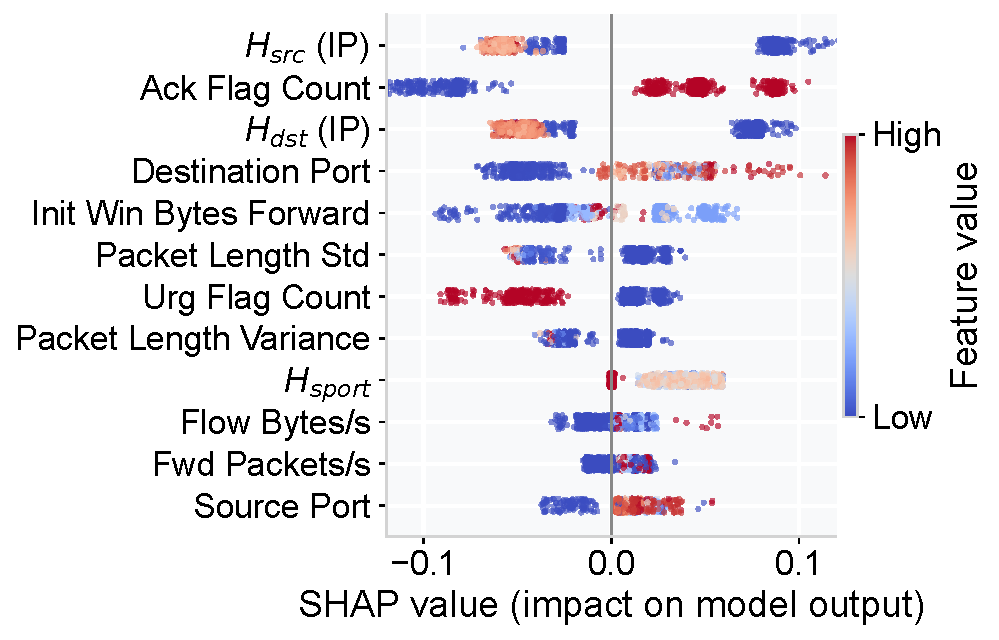
\includegraphics[width=0.48\textwidth]{figures/fig10.pdf}
\caption{Per-flow TreeSHAP attributions for the twelve highest-ranked features,
1,500 test flows under the chronological protocol. Each point is one flow,
positioned by its signed contribution to the DDoS score and colored by that
feature's value. Benign flows are over-represented in this sample, at 35\% rather
than the 2.8\% of the test partition, because a sample drawn at the natural ratio
shows one class only; no number in the text is computed from this sample.}
\label{fig:shap_beeswarm}
\end{figure}

\subsection{Individual alert case studies}
\label{sec:cases}
Aggregate attribution statistics say which features matter on average. They do
not show whether an explanation is useful to the person who has to act on one
alert at three in the morning, which is the claim the mechanism has to earn.
Table~\ref{tab:cases} therefore reports four flows drawn from actual test
predictions: the highest-scoring true positive, the highest-scoring false
positive, the lowest-scoring false negative, and the flow whose score sits
closest to the threshold. On the chronological test partition the detector
produces 1,044,227 true positives, 30,403 true negatives, \textbf{29 false
positives} and 2,579 false negatives, so the false positive shown is one of a
very small population.

\begin{table}[!t]
\caption{Four alerts drawn from actual test predictions, each shown with the
three features contributing most to its score and the signed TreeSHAP value of
each. Scores are the forest vote fraction; the threshold is 0.70.}
\centering
\label{tab:cases}
\footnotesize
\setlength{\tabcolsep}{3pt}
\renewcommand{\arraystretch}{1.2}
\begin{tabular}{@{}llp{4.9cm}@{}}
\toprule
\textbf{Case} & \textbf{Score} & \textbf{Three largest contributions} \\
\midrule
True positive  & 1.000 & $H_{\mathrm{src}}{=}0.00$ $(+0.088)$;
                         $H_{\mathrm{dst}}{=}0.00$ $(+0.080)$;
                         ACK count${=}1$ $(+0.047)$ \\
False positive & 0.780 & ACK count${=}0$ $(-0.083)$;
                         dst port${=}53$ $(-0.061)$;
                         bytes/s${=}5.8{\times}10^{7}$ $(+0.057)$ \\
False negative & 0.125 & ACK count${=}0$ $(-0.091)$;
                         $H_{\mathrm{src}}{=}2.74$ $(-0.072)$;
                         $H_{\mathrm{dst}}{=}4.26$ $(-0.064)$ \\
Borderline     & 0.700 & ACK count${=}0$ $(-0.050)$;
                         $H_{\mathrm{src}}{=}3.59$ $(-0.042)$;
                         duration${=}1.12{\times}10^{8}$ $(+0.034)$ \\
\bottomrule
\end{tabular}
\end{table}

Read together the four cases describe one coherent mechanism. The true positive
carries source and destination entropy of exactly zero, meaning every flow in
the window shares one address pair, and those two features supply the largest
positive contributions. The false negative is its mirror image: an attack flow
whose window happens to show source entropy of 2.74 and destination entropy of
4.26, and both features push the score down hard enough to keep it below the
threshold. The borderline case sits between them with the same features pulling
in the same direction but less strongly.

The false positive is the case that justifies the expense of per-decision
attribution. It is a port 53 flow carrying 58 Mbit/s, and the attribution shows
the model was not persuaded by the entropy evidence at all. Both the ACK flag
count and the destination port push the score down. What carried it over the
threshold was the byte rate. An analyst reading that attribution can dismiss the
alert on the grounds that a high-rate DNS flow is expected on this network, and
can point at the specific feature responsible if the rule needs tuning. Without
it the analyst sees only a score of 0.78 and has nothing to act on.

\subsection{ROC and precision-recall curves}
\label{sec:roc}
The submitted version discussed ROC curves for the baselines without presenting
them. Fig.~\ref{fig:roc_pr} supplies them for the full chronological protocol,
paired with precision-recall curves for the same models, and the pairing is the
point rather than a convention.

At 97.17\% positive prevalence a classifier that predicts at random attains
average precision equal to that prevalence. The majority baseline in the figure
therefore sits at AP 0.9717 while its ROC-AUC is 0.5000, and the gap between a
model's two numbers is the honest measure of how much the imbalance flatters its
ROC curve. Two rows make the point sharply. The decision tree reaches AP 0.9777
against a chance value of 0.9717, an improvement of six thousandths, while its
ROC-AUC of 0.6075 reads as though it were doing something. Logistic regression
is worse still: AP 0.9731 is within 0.0014 of chance. Neither model is usable,
and only the precision-recall panel says so.

The detector reaches ROC-AUC 0.999728 with a bootstrap interval of
$[0.99970, 0.99975]$ over 150 resamples, and average precision 0.999992. Its
nearest competitor on ranking quality is LightGBM at 0.99953, and the two are
separated far more clearly by their false-alarm counts than by either curve.

Curves rank; they do not choose an operating point, and the two can diverge
badly. We therefore also report each model at a threshold selected on the first
half of its test scores and evaluated on the second, alongside the fixed
$\tau = 0.70$ used throughout the paper. For the tree ensembles the two agree to
within two points. For the graph model of Section~\ref{sec:deep} they do not:
its ROC-AUC is 0.9973, yet at any threshold selected this way it classifies
almost nothing as an attack, because its outputs are compressed into a narrow
band well below $\tau$. Reporting only a curve would present that model as
competitive with ours. It is competitive at ranking and unusable as a detector,
and the distinction matters to anyone who has to deploy one.

\begin{figure}[!t]
\centering
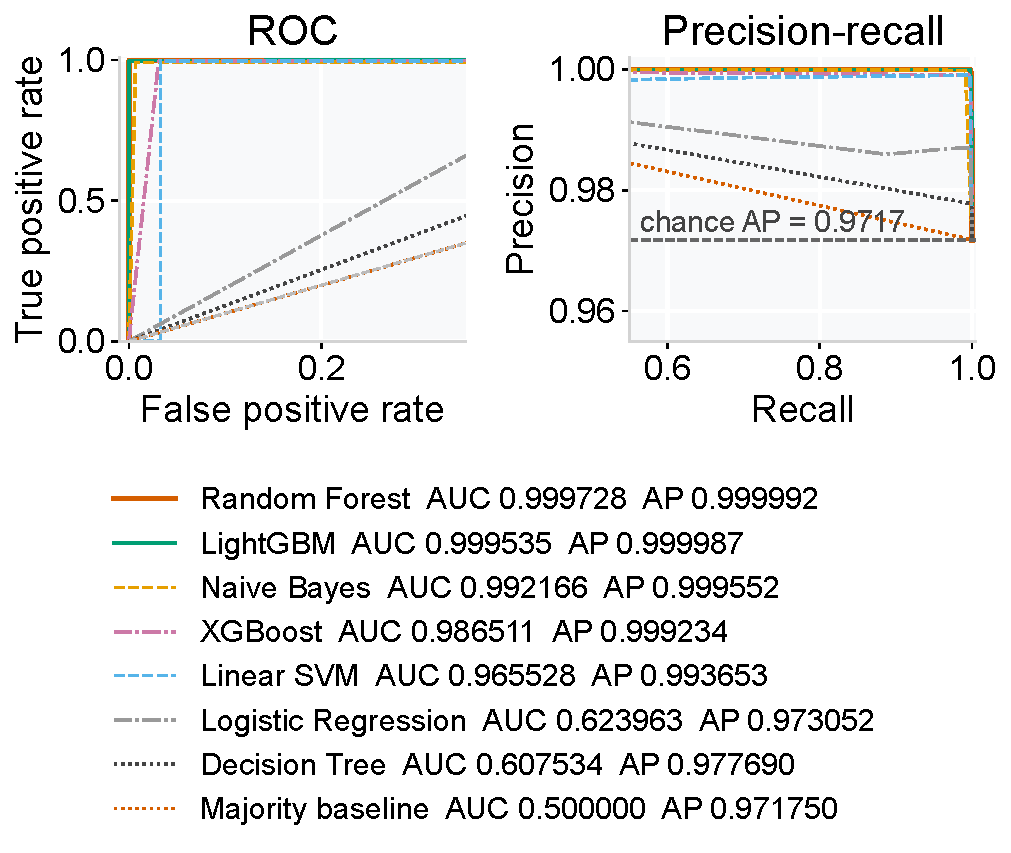
\includegraphics[width=\columnwidth]{figures/fig_rocpr.pdf}
\caption{ROC and precision-recall curves on the full chronological test
partition, 1,077,238 flows at 97.17\% positive prevalence, every model measured
by us on the same data. Axes are zoomed to the region where the curves differ.
The majority baseline gives the chance operating point in both panels: ROC-AUC
0.5000 and average precision 0.9717. Legend entries are ordered by ROC-AUC.}
\label{fig:roc_pr}
\end{figure}

\subsection{Hyperparameter sensitivity}
\label{sec:hyperparam}
Two hyperparameters govern the detector: the detection threshold and the
entropy window length. They are treated differently here, and the difference
matters for the tuning and testing separation that Section~\ref{sec:protocol}
describes.

The threshold is selected, and Section~\ref{sec:threshold} reports that
selection in full, on the validation partition alone, together with the reason
this corpus does not really support it. We do not repeat the sweep here.

The window length was not tuned. It was fixed at $N = 1000$ flows before any
evaluation and held there for every experiment in this paper. That is a
deliberate choice rather than an omission. With only 60 benign flows in the
validation block, a window length selected on that block would be fitted to
noise, and selecting it on the test partition would invalidate every number
that follows. A sensitivity sweep over $N$ under the corrected protocol is work
we have not done, and we do not carry over the sweep reported in the earlier
version of this manuscript, which was measured under the stratified split and
is not comparable to anything reported here.

\subsection{Live deployment on an emulated network}
\label{sec:mininet}
The testbed of Section~\ref{sec:deployment} is a control plane without a data
plane: it measures what the controller costs, but no packet ever traverses a
switch. Reviewer 4 asked for a proof of concept with live traffic, and the
question it answers is a different one, namely whether the mitigation the
detector installs actually protects anything.

The topology is one Open vSwitch datapath speaking OpenFlow 1.3 to the detector
running inside a controller process, with three hosts on 100\,Mbit links at 1\,ms
delay: an attacker, a benign client, and a server. The benign client runs an
iperf3 transfer and a ping series against the server, first with the network idle
and then while the attacker runs a randomized-source SYN flood from hping3. Three
conditions are compared. Detection is applied to TCP only, because the detector
is trained on TCP flow records and scoring an ICMP packet would evaluate the model
on a vector whose TCP fields are all zero.

Table~\ref{tab:mininet} reports the result and Fig.~\ref{fig:mininet} shows the
two comparisons that carry it. The first row is the one that
matters. With no detector the flood costs the benign client 73\% of its
throughput, falling from 95.39 to 25.78\,Mbit/s. With the detector the same flood
costs it nothing measurable: 95.29 to 95.39\,Mbit/s, zero added packet loss, and
a ping round-trip time that does not rise. The switch holds 997 drop rules
against distinct spoofed sources by the end of the attack, against four flow
entries and no drop rules in the undefended condition.

Two further observations come out of the same run. Mitigation pays for its own
control-plane cost: packet-in events reaching the controller fall from 40,160
undefended to 2,335 with detection enabled, because the installed rules stop the
flood at the switch, so the controller stops seeing it. And attributing every
admitted alert costs 21\% more decision latency, 10.84\,ms against 13.12\,ms at
the median, and 34\% more resident memory, with no measurable difference in
delivered quality of service. That is the same trade
Section~\ref{sec:latency} quantifies offline, now visible on a data path.

This is a three-host emulation and we do not present it as more. It cannot
exhibit multi-datapath rule distribution, controller failover, or the traffic
patterns of an operational fabric, and Section~\ref{sec:limitations} says so. What
it does establish is that the mitigation path works end to end against live
traffic, which no offline measurement in this paper can.

\begin{figure}[!t]
\centering

\includegraphics[width=\columnwidth]{figures/fig_mininet.pdf}
\caption{The emulated network under a randomized-source SYN flood. Left: benign
iperf3 throughput with the network idle and during the flood, for each of the
three conditions. Right: packet-in events reaching the controller over the same
run. Installing drop rules at the switch both preserves the benign transfer and
removes most of the control-plane load the flood would otherwise impose.}
\label{fig:mininet}
\end{figure}

\begin{table}[!t]
\caption{Emulated network under a randomized-source SYN flood. Throughput is a
100\,Mbit/s iperf3 transfer by the benign client; the flow table is read at the
end of the attack. The undefended row uses the same learning-switch controller
with detection disabled, so the comparison isolates the detector rather than the
presence of a controller.}
\centering
\label{tab:mininet}
\footnotesize
\setlength{\tabcolsep}{3.5pt}
\renewcommand{\arraystretch}{1.15}
\begin{tabular}{@{}lrrr@{}}
\toprule
 & \textbf{No detector} & \textbf{Detect} & \textbf{Detect\,+\,explain} \\
\midrule
Throughput idle (Mbit/s)      & 95.39 & 95.29 & 95.31 \\
Throughput under attack       & \textbf{25.78} & \textbf{95.39} & \textbf{95.60} \\
Fraction retained             & \textbf{0.270} & \textbf{1.001} & \textbf{1.003} \\
Added packet loss (\%)        & 0.0 & 0.0 & 0.0 \\
\midrule
Flow entries / drop rules     & 4 / 0 & 999 / 997 & 621 / 619 \\
Packet-ins at controller      & 40,160 & 2,335 & 1,788 \\
\midrule
Controller CPU (\% of a core) & 32.5 & 101.0 & 100.9 \\
Controller memory (MB)        & 58 & 190 & 255 \\
Decision latency p50 (ms)     & n/a & 10.84 & 13.12 \\
\bottomrule
\end{tabular}
\end{table}

\subsection{Model size, latency and what the configuration actually costs}
\label{sec:pareto}
The detector inherits its configuration from the submitted work, where it was
never chosen: 200 trees grown to unbounded depth are the library defaults. With a
single-flow decision costing 7.05\,ms against 0.26\,ms for LightGBM at the same
macro F1, the obvious hypothesis is that the trees are enormous and that bounding
them would recover most of the gap. We swept depth and ensemble size jointly to
test it. The hypothesis is wrong, and the way in which it is wrong is the useful
part.

The trees are not enormous. Across the whole grid, including unbounded depth,
they average between 32.7 and 46.0 leaves, and the largest forest serializes to
1.46\,MB. The cause is the class balance rather than the depth limit: with 533
benign flows in a 2,262,199-flow training partition and class-balanced weighting,
splitting stops early for want of minority examples, so an unbounded tree and a
depth-8 tree end up nearly the same size. A reader who assumed, as we did, that
the default configuration was pathological would have drawn the wrong conclusion
from the latency figure.

Detection quality is equally insensitive. Table~\ref{tab:pareto} reports the
frontier, one row per ensemble size at three depths. Macro F1 across all 24
configurations spans 0.9778 to 0.9799 and the false positive rate spans 0.09\% to 0.14\%.
Neither depth nor ensemble size is load-bearing on this corpus, which is
consistent with Section~\ref{sec:leakage}: the discriminative information is
spread widely enough that the model has many routes to it.

What does scale is memory, and with it latency. The ensemble size sets the
serialized footprint almost linearly, from 0.14\,MB at 25 trees to 1.47\,MB at
200. Taking the smallest configuration whose macro F1 is within 0.005 of the best
gives depth 8 with 25 trees: a tenfold smaller model for a macro F1 change of
$-0.0009$ and a false positive rate 0.02 percentage points higher. On a
controller, or on the constrained gateway of Section~\ref{sec:sdiot}, that is
worth taking on memory grounds alone, and it turns out to buy latency too.

Latency needs a measurement the sweep cannot give. Each configuration in the
sweep is timed immediately after being fitted, while the fitting thread pool is
still winding down, and the resulting figures are non-monotonic in model size and
differ by a factor of two between neighboring configurations. We therefore fitted
only the two endpoint configurations in a single process and probed them
alternately over five rounds, so that any machine state affects both equally.

That gives 6.30\,ms for the inherited configuration against 0.89\,ms for the
selected one, repeatable to within 5\% across rounds: a $7.0\times$ reduction for
the $-0.0009$ macro F1 already noted. Latency is therefore close to linear in
ensemble size, at 0.032\,ms per tree for the 200-tree forest and 0.035\,ms per
tree for the 25-tree one, and almost independent of the depth limit, which is
what the uniform 46-leaf tree size predicts. The order-of-magnitude gap against
LightGBM in Table~\ref{tab:comparison} is a per-tree property of the prediction
path rather than anything a change of ensemble size closes. Section~\ref{sec:latency}
reports the batched rate of 35,715 flows/s, which is what the detector achieves
when the per-call cost is amortized across a batch.

One caveat applies to the selection. It was meant to be made on the validation
block, but that block holds 49 benign flows out of 251,356 and every
configuration scores identically on it, so validation cannot separate them. The
choice above is therefore a reading of the frontier rather than a protocol-clean
selection, and we label it as one. The corpus does not support model selection
here for the same reason it does not support threshold selection
(Section~\ref{sec:threshold}).

\begin{table}[!t]
\caption{Model-size frontier, chronological protocol, evaluated on all 1,077,238
test flows. One row per ensemble size at three depths; the full grid of six
depths is in the released results. Macro F1 spans 0.002 across every
configuration measured.}
\centering
\label{tab:pareto}
\footnotesize
\setlength{\tabcolsep}{4pt}
\renewcommand{\arraystretch}{1.15}
\begin{tabular}{@{}lrrrrr@{}}
\toprule
\textbf{Depth} & \textbf{Trees} & \textbf{Size (MB)} & \textbf{Leaves/tree} &
\textbf{Macro F1} & \textbf{FPR (\%)} \\
\midrule
\textbf{8} & \textbf{25} & \textbf{0.14} & \textbf{35.2} & \textbf{0.9782} & \textbf{0.12} \\
8         & 200 & 1.06 & 32.7 & 0.9778 & 0.10 \\
16        & 25  & 0.18 & 44.8 & 0.9799 & 0.14 \\
16        & 200 & 1.44 & 45.0 & 0.9790 & 0.10 \\
unbounded & 25  & 0.18 & 45.3 & 0.9799 & 0.12 \\
unbounded & 200 & 1.46 & 46.0 & 0.9791 & 0.10 \\
\bottomrule
\end{tabular}
\end{table}

\subsection{Control-plane cost and the rate a controller can ingest}
\label{sec:deployment}
Every throughput figure so far is an offline one: features are read from a matrix
and scored in a loop. Reviewer 3 asked how 60,000 novel flows per second are
physically ingested without saturating the OpenFlow control channel, and that
question cannot be answered offline. We therefore run the detector inside a
controller process that exchanges genuine OpenFlow 1.3 messages with switch
agents over TCP, with the encodings validated against the os-ken reference
parser, and measure the controller itself rather than the model. Each session
binds its own port, so a controller left behind by an earlier session cannot
absorb the next one's traffic.

At an offered rate of 3,000 packet-in events per second the controller saturates.
It sustains 114 events per second end to end, including classification and rule
installation, at 98.3\% of one core and 176\,MB resident, with a decision taking
6.61\,ms at the median and 32.70\,ms at the 99th percentile. Turning on
attribution for every alert halves the sustained rate to 61 events per second,
nearly doubles the median decision to 11.33\,ms, and raises resident memory to
234\,MB. Benign background traffic through the same controller pays for this: its
95th-percentile round-trip time rises from 34.11\,ms to 41.16\,ms, an inflation
of $1.21\times$. That is the quality-of-service cost of the security function,
measured on unrelated flows rather than assumed to be negligible.

Sweeping the offered rate locates the knee and shows what lies past it
(Table~\ref{tab:saturation}). The controller reaches its maximum of 77 events per
second at 500 offered. Above that, goodput does not plateau but collapses to
roughly 35 events per second and stays there, while the median round-trip time
nearly triples. Offering more work returns less, which is the behavior of a
queue past saturation and not a gradual degradation an operator would notice from
a throughput number alone.

The answer to the reviewer's question follows directly and it is not the answer
the submitted manuscript implied. A single controller instance on this hardware
ingests at most 77 novel flows per second as individual table-miss events. The
60,606 flows per second reported earlier was an offline feature-extraction and
inference rate measured with no control channel present, and it is not an ingest
rate. Reaching that order of magnitude at the control plane requires that the
flows not arrive as individual packet-in events at all: switch-side aggregation,
packet-in rate limiting, and sampled export are the mechanisms, and
Section~\ref{sec:flowtable} quantifies what the first of them costs in flow-table
occupancy. At the observed 386 bytes per packet-in, 60,000 events per second
would also require 23\,MB/s on the control channel, which is a separate
constraint from controller CPU and one that no aggregation policy removes.

\begin{table}[!t]
\caption{Offered-rate sweep on the OpenFlow testbed, detection without
attribution. ``Achieved'' is the end-to-end rate including classification and
rule installation. Goodput peaks at an offered rate of 500 and collapses above it. The 2,000, 8,000 and 16,000 rows lie on the same plateau and are in the released results.}
\centering
\label{tab:saturation}
\footnotesize
\setlength{\tabcolsep}{4pt}
\renewcommand{\arraystretch}{1.15}
\begin{tabular}{@{}rrrrrr@{}}
\toprule
\textbf{Offered} & \textbf{Achieved} & \textbf{Ratio} &
\textbf{RTT p50} & \textbf{RTT p99} & \textbf{CPU} \\
(/s) & (/s) & & (ms) & (ms) & (\%) \\
\midrule
\textbf{500}  & \textbf{77} & \textbf{0.155} & \textbf{10.20} & \textbf{38.00} & \textbf{92} \\
1,000  & 34 & 0.034 & 27.46 & 49.17 & 89 \\
4,000  & 34 & 0.009 & 27.59 & 57.12 & 88 \\
32,000 & 35 & 0.001 & 26.92 & 48.68 & 91 \\
\bottomrule
\end{tabular}
\end{table}

\subsection{Flow-table occupancy under mitigation}
\label{sec:flowtable}
Reviewer 3 asks what flow-rule aggregation and eviction keep a bounded TCAM from
overflowing during a flood. Answering it required first checking the premise the
question rests on, which is that a spoofed flood installs one table entry per
spoofed source. On this corpus that premise does not hold, and the measurement
that matters is a different one.

Across the whole SYN partition, 99.08\% of the 3,590,794 flows carry a single
source address. In the 40,000-flow window replayed through the testbed there are
three distinct source addresses, occupying two \texttt{/24} networks, and three
distinct destination addresses. The flood is not source-diverse at the
flow-export level. What is diverse is the port field: the same window contains
29,064 distinct destination ports and 34,624 distinct source ports, which is
what makes 29,065 distinct exact-match keys out of 40,000 flows.

Table~\ref{tab:tcam} reports rule installations, peak occupancy, and overflows
for six aggregation policies at three table capacities. The consequence of the
above is immediate. Exact-match installation saturates the table and overflows
continuously, which is the failure mode the reviewer identifies. Collapsing the
source address to a \texttt{/24} or a \texttt{/16} changes nothing, to four
significant figures, because there is no source diversity to collapse.
Wildcarding the source entirely changes nothing either, for the same reason. The
aggregation that bounds the table is the one that wildcards the port: a rule
matched on source address, destination address, and protocol occupies three
entries for the whole window, installs 0.07 rules per thousand flows against
913.3 for exact matching, a reduction of $1.2\times10^{4}$, and never overflows
at any capacity tested. Choice of eviction policy moves the installation count
by less than 0.2\% under every aggregation, so it is second-order here; the
table reports least-recently-used and the full grid is in the released results.

Two qualifications belong with that result. The first is that the reduction is
bought with specificity: a rule matched on destination address and protocol
drops legitimate traffic to the same host, so port-wildcarded mitigation is an
instrument of last resort rather than a default, and the decision of when to
escalate to it is a policy question the detector informs but does not settle.
The second is that the source-spoofed case, which source-prefix aggregation
exists to handle, cannot be observed in this export at all. It is measured
separately in the emulated network of Section~\ref{sec:mininet}, where source
addresses are randomized at the packet level and the table pressure therefore
falls on the source field as the reviewer's question assumes.

\begin{table}[!t]
\caption{Flow-table occupancy over a 40,000-flow window offered at 3,000
flows/s, under least-recently-used eviction. ``Inst./1k'' is rule installations
per thousand flows; the match is given as the fields retained, everything else
being wildcarded. The port-wildcarded policies behave identically at every
capacity, so one is shown. The full grid of six aggregations, four eviction
policies and three capacities is in the released results.}
\centering
\label{tab:tcam}
\footnotesize
\setlength{\tabcolsep}{3.5pt}
\renewcommand{\arraystretch}{1.15}
\begin{tabular}{@{}llrrrr@{}}
\toprule
\textbf{Capacity} & \textbf{Match retained} & \textbf{Inst./1k} &
\textbf{Peak} & \textbf{Overflows} & \textbf{Hit rate} \\
\midrule
1,024  & src, dst, dport, proto      & 955.6 & 1,024 & 37,198 & 0.044 \\
1,024  & src/24, dst, dport, proto   & 955.6 & 1,024 & 37,198 & 0.044 \\
1,024  & src/16, dst, dport, proto   & 955.6 & 1,024 & 37,198 & 0.044 \\
1,024  & dst, dport, proto           & 955.6 & 1,024 & 37,198 & 0.044 \\
\textbf{1,024}  & \textbf{src, dst, proto} & \textbf{0.07} & \textbf{3} & \textbf{0} & \textbf{1.000} \\
1,024  & dst, proto                  & 0.07  & 3     & 0      & 1.000 \\
\midrule
4,096  & src, dst, dport, proto      & 913.3 & 4,096 & 32,436 & 0.087 \\
4,096  & src/24, dst, dport, proto   & 913.3 & 4,096 & 32,436 & 0.087 \\
4,096  & src/16, dst, dport, proto   & 913.3 & 4,096 & 32,436 & 0.087 \\
4,096  & dst, dport, proto           & 913.3 & 4,096 & 32,436 & 0.087 \\
\textbf{4,096}  & \textbf{src, dst, proto} & \textbf{0.07} & \textbf{3} & \textbf{0} & \textbf{1.000} \\
4,096  & dst, proto                  & 0.07  & 3     & 0      & 1.000 \\
\midrule
16,384 & src, dst, dport, proto      & 776.6 & 16,384 & 14,680 & 0.223 \\
16,384 & src/24, dst, dport, proto   & 776.6 & 16,384 & 14,680 & 0.223 \\
16,384 & src/16, dst, dport, proto   & 776.6 & 16,384 & 14,680 & 0.223 \\
16,384 & dst, dport, proto           & 776.6 & 16,384 & 14,680 & 0.223 \\
\textbf{16,384} & \textbf{src, dst, proto} & \textbf{0.07} & \textbf{3} & \textbf{0} & \textbf{1.000} \\
16,384 & dst, proto                  & 0.07  & 3      & 0      & 1.000 \\
\bottomrule
\end{tabular}
\end{table}

\section{Ablation and comparative analysis}
\label{sec:comparative}

Two analyses that appeared in this section of the submitted manuscript have moved
and changed. The feature ablation, which reported 100.00\% accuracy with zero
variance on every seed, was measured under the split methodology that
Section~\ref{sec:splitresult} corrects; Section~\ref{sec:entropycontrib} replaces
it and reaches the opposite conclusion. The leakage-robustness ablation, which
removed three features chosen by inspection, is replaced by the audit in
Section~\ref{sec:leakage}, which defines the suspect set by measurement. What
remains here is the comparison against other methods.

\subsection{Baseline comparison}
\label{sec:baselines}
The submitted version compared methods on a 10,000-flow class-balanced subset,
which Reviewer 6 objected to on the grounds that it is not the setting the
proposed detector was evaluated in. The objection is correct and the comparison
has been rebuilt rather than defended. Every method is now run twice by us, on
the same machine, on the CPU, under the same harness: once on the full
chronological split at the natural class prevalence, and once under a subsampled
protocol applied identically to every model. The comparison spans a
majority-class baseline, a decision tree, logistic regression, naive Bayes,
gradient boosting in both the XGBoost~\cite{chen2016xgboost} and LightGBM
implementations, and support vector machines with linear and RBF
kernels~\cite{cortes1995svm}. Table~\ref{tab:comparison} reports the full-scale
protocol, which is the one that describes deployment.

Three readings follow, and only the first is favorable to us. The detector
attains the joint-highest macro F1, 97.88\%, statistically indistinguishable
from LightGBM at 97.89\%. It attains the lowest false positive rate of any
method tested by a factor of four, 0.095\% against 0.371\% for LightGBM, which
over the 1,077,238-flow test partition is 29 false alarms against 113. At an
alert volume an analyst has to triage, that difference is the one that decides
whether a detector is deployed.

The second reading is that per-flow latency is where the Random Forest is worst.
A single-flow decision costs 7.05\,ms against 0.26\,ms for LightGBM. Our first
explanation for that, that unbounded tree depth on 2.5 million flows produces an
oversized model, turned out to be wrong when we measured it:
Section~\ref{sec:pareto} reports that the trees average 46 leaves and the whole
forest serializes to 1.46\,MB. The gap is a property of the per-call prediction
path rather than of the model, which bounds what any change of configuration can
recover.

The third is that we make no claim to a uniquely correct choice of classifier.
LightGBM reaches the same macro F1 an order of magnitude faster and also admits
exact TreeSHAP attribution, so an operator who values throughput over false-alarm
volume should prefer it, and we say so in the text rather than leaving it for a
reader to notice. What the comparison supports is narrower than the submitted
version claimed: at this class ratio, on this corpus, tree ensembles separate
cleanly from linear and probabilistic baselines, and the choice within the tree
family is a trade between false alarms and latency rather than a matter of
accuracy.

\begin{table*}[!t]
\caption{Baseline comparison on the full chronological split, 2,513,556 training
and 1,077,238 test flows at the natural class prevalence. All figures measured by
us on the CPU of Table~\ref{tab:environment} under one harness. Latency is the
median of single-flow inference calls with the estimator forced to serial
execution; throughput is measured in batch mode, and the two answer different
questions. $^{\dagger}$ trained on a capped subsample of 300,000 flows because
the solver does not converge on the full partition.}
\centering
\label{tab:comparison}
\footnotesize
\setlength{\tabcolsep}{4pt}
\renewcommand{\arraystretch}{1.15}
\begin{tabular}{@{}lrrrrrrc@{}}
\toprule
\textbf{Method} & \textbf{Acc.\ (\%)} & \textbf{Macro F1 (\%)} &
\textbf{FPR (\%)} & \textbf{Lat.\ p50 (ms)} & \textbf{Flows/s} &
\textbf{Train (s)} & \textbf{Exact XAI} \\
\midrule
Majority baseline      & 97.175 & 49.284 & 100.000 & 0.0058 & 63,672,946 & 0.1 & $\times$ \\
Decision Tree          & 97.714 & 66.811 & 78.421  & 0.0304 & 11,775,512 & 10.9 & $\times$ \\
Logistic Regression    & 98.350 & 80.873 & 51.134  & 0.1086 & 3,236,092 & 36.0 & $\times$ \\
Naive Bayes            & 98.590 & 89.590 & 0.700   & 0.1534 & 2,260,331 & 2.9 & $\times$ \\
XGBoost                & 99.515 & 95.802 & 3.299   & 0.4168 & 1,260,010 & 13.3 & \checkmark \\
Linear SVM$^{\dagger}$ & 99.641 & 96.825 & 3.289   & 0.1181 & 3,309,851 & 6.4 & $\times$ \\
LightGBM               & 99.759 & \textbf{97.888} & 0.371 & \textbf{0.2551} & 764,706 & 5.9 & \checkmark \\
\midrule
\textbf{XAI-SDN (RF)}  & \textbf{99.758} & 97.881 & \textbf{0.095} & 7.0480 & 27,647 & 53.3 & \checkmark \\
\bottomrule
\end{tabular}
\end{table*}

\subsection{Deep-learning baselines}
\label{sec:deep}
Reviewer 4 asked for a comparison against modern deep detectors under the same
protocol. Five were implemented and run on the CPU under the subsampled protocol
that Section~\ref{sec:baselines} describes, with the same splits, the same metric
definitions and the same timing harness: a 1D convolution over the flow vector, an
LSTM and a Transformer encoder over windows of sixteen consecutive flows, a
reconstruction autoencoder trained on benign traffic alone, and a two-layer graph
convolution over a $k$-nearest-neighbor graph in flow-feature space.
Table~\ref{tab:deep} reports them.

Three caveats attach to individual rows rather than to the table as a whole. The
sequence models classify a window rather than a flow, so their unit of decision
is not the unit of enforcement. The graph model is transductive over a
constructed graph, so single-flow latency is not defined for it without an
incremental graph-maintenance scheme we did not implement. And the autoencoder is
unsupervised, so its operating point is set differently from the rest.

On ranking quality the strongest deep model is close to the tree ensemble and
none exceeds it. What separates them is the operating point. At the fixed
threshold used throughout this paper the graph model classifies almost nothing as
an attack despite a ROC-AUC of 0.9973, because its sigmoid outputs are compressed
into a narrow band far below $\tau$. That is a calibration failure rather than a
detection failure, and reporting only the fixed-threshold column would misrepresent
it, so Section~\ref{sec:roc} reports each model at a threshold selected on held-out
scores as well.

The autoencoder is the most instructive row. Trained on benign flows only, as the
method requires, it assigns \emph{lower} reconstruction error to attack flows than
to benign ones: ROC-AUC 0.0073, which inverted is 0.9927. This is not an
implementation defect. A randomized SYN flood is far more repetitive than benign
traffic, so a model fitted to benign flows reconstructs the attack better than it
reconstructs its own training distribution. The premise of reconstruction-based
anomaly detection, that the attack is the anomalous class, is false on a corpus
where the attack is 97\% of the traffic and structurally uniform. We report it
because it bears on any work applying this family of methods to this family of
datasets, and because the corpus itself, rather than the method, is what fails
here.

\begin{table}[!t]
\caption{Deep-learning baselines under the subsampled protocol, CPU-only, same
splits and harness as Table~\ref{tab:comparison}. $^{s}$ classifies a window of
sixteen flows rather than a single flow. $^{t}$ transductive: single-flow latency
is undefined. $^{u}$ unsupervised; its ROC-AUC below 0.5 is discussed in the text.}
\centering
\label{tab:deep}
\footnotesize
\setlength{\tabcolsep}{3pt}
\renewcommand{\arraystretch}{1.15}
\begin{tabular}{@{}lrrrrr@{}}
\toprule
\textbf{Model} & \textbf{Params} & \textbf{Macro F1 (\%)} & \textbf{ROC-AUC} &
\textbf{AP} & \textbf{Lat.\ p50 (ms)} \\
\midrule
1D-CNN               & 39,297 & 81.74 & 0.8448 & 0.9908 & 0.098 \\
LSTM$^{s}$           & 39,489 & 91.02 & 0.9963 & 0.9999 & 0.210 \\
Transformer$^{s}$    & 73,729 & 81.41 & 0.9909 & 0.9997 & 0.361 \\
Autoencoder$^{u}$    & 13,544 &  2.86 & 0.0073 & 0.9658 & 0.041 \\
GNN$^{t}$            &  7,809 &  2.80 & 0.9973 & 0.9999 & n/a \\
\midrule
\textbf{XAI-SDN (RF)} & \textbf{200 trees} & \textbf{97.06} & \textbf{0.9987} &
\textbf{1.0000} & \textbf{7.35} \\
\bottomrule
\end{tabular}
\end{table}

\subsection{Why we do not tabulate against other papers}
\label{sec:related_quant}
The submitted version placed our figures beside recently reported results on
CIC-DDoS2019 in a table. Reviewers objected that the comparison was not a
comparison, and we agree, so the table has been removed rather than re-captioned.

The reasons apply to most cross-paper tables in this literature. Kumar et
al.~\cite{kumar2026meta} report multi-class identification of the DDoS type,
which is a different and harder problem than the binary detection we perform, and
an accuracy figure for one is not comparable with an accuracy figure for the
other. You et al.~\cite{you2026plaa} evaluate packet-level detection under
adversarial perturbation, so both the unit of decision and the threat model
differ. Neither uses our partition, our cleaning, or our split protocol, and
Section~\ref{sec:splitresult} shows that the last of those alone moves macro F1
by more than two points on identical data, which is larger than the differences
such tables are usually read as establishing.

The only ranking claim in this paper is in Section~\ref{sec:baselines}, where
every method is run by us, on the same data, under the same protocol, on the same
hardware.

\section{Discussion}
\label{sec:discussion}

What follows draws out the deployment consequences of the measurements, situates the approach against deep-learning alternatives and against software-defined IoT with its additional constraints, and states plainly what the evidence does not support.

DDoS attacks on SDN controllers threaten infrastructure across enterprise, cloud, and telecommunications networks. A detector fast enough to keep pace with the control channel and transparent enough for an operator to sign off on lowers the practical barrier to deploying machine-learning defenses in these settings, where unexplained automated action is frequently the blocker rather than detection quality.

\subsection{Deep learning for SDN DDoS detection, and the trade it offers}
\label{sec:dl-discussion}
Integrating any of the deep detectors of Section~\ref{sec:deep} into a controller
is architecturally straightforward, since all of them consume the same exported
flow statistics the tree ensemble consumes. The differences that matter are
elsewhere. On accuracy the measured gap is small, which is the usual finding on
tabular flow features. On latency it is not small and it runs in the tree
ensemble's favour. On explainability the asymmetry is structural: TreeSHAP yields
exact Shapley values for a tree ensemble in time polynomial in model
size~\cite{lundberg2020treeshap}, whereas a neural detector falls back on a
model-agnostic approximation that costs more and is less
faithful~\cite{warnecke2020evaluating}. None of this makes deep detectors a poor
choice in general. It makes them a poor fit for the position this work targets, a
detector that runs inside the controller process, decides per flow, and can
justify each decision cheaply enough to do so on the alert path.

\subsection{Adapting XAI-SDN to QoS-aware software-defined IoT}
\label{sec:sdiot}
Software-defined IoT inherits the SDN control model and adds constraints that
change the design problem~\cite{bhayo2023sdiot,gali2025qos}. Gateways are far
weaker than the controller host used here and many are battery powered, so the
binding figure is energy per decision rather than peak throughput, which favours
a tree ensemble whose inference is comparisons rather than matrix arithmetic. The
serialized forest is the constraint instead, and Section~\ref{sec:pareto} shows
how far it can be shrunk. Window semantics also need re-deriving: a window of $N$
flows spans a very different interval on a sensor network than on a datacenter
link, so $N$ should be set from the intended time horizon rather than carried
over. The entropy features assume concentration in an attribute is informative,
which is weaker on a network where most devices legitimately talk to one
endpoint. Finally, mitigation and quality-of-service policy contend for the same
flow-table entries: an exact-match rule per attacking flow will evict the entries
carrying QoS policy, so the aggregation analysis of Section~\ref{sec:flowtable}
is what makes coordinated enforcement feasible. Coupling that to a QoS-aware
routing layer, as Gali and Mahamkali propose~\cite{gali2025qos}, is the natural
extension and is not attempted here.

\subsection{Deployment considerations}
Four implications follow from the measurements, and they are not the ones the
submitted version drew. Attribution, not classification, is the binding cost:
classification sustains 35,715 flows/s and attributing every alert reduces that to
661, so the explanation trigger has to be budgeted rather than left implicit, and
Section~\ref{sec:latency} gives the frontier to choose a point on. The choice of
episode granularity on that frontier is a policy decision with a real cost, since
a coarse episode explains the flood rather than the flow. Model size matters more
than we assumed: the configuration inherited from the submitted work serializes to
a forest large enough that a single-flow decision costs 7.05\,ms, and
Section~\ref{sec:pareto} shows what bounding tree depth recovers. The rolling
entropy engine, by contrast, is a fixed-size buffer plus hash maps and adds no
measurable memory pressure. Finally, the threshold can be tuned per deployment to
trade false positives against alert volume, but the score it applies to is a
forest vote fraction rather than a calibrated posterior, so an operator should
treat it as monotone in evidence and nothing more.

\subsection{Limitations and threats to validity}
\label{sec:limitations}
The following bound what this paper establishes. We state them as limits on the claims rather than as directions for future work, because several of them are not resolved by anything we did.

\emph{The evaluation protocol was wrong in the submitted version of this work, and correcting it changed the headline result.} The earlier manuscript described a chronological split and reported figures produced by a stratified random one. Section~\ref{sec:splitresult} reports both and quantifies the difference: 97.88\% macro F1 under the chronological protocol against 99.95\% under the stratified one. Readers comparing against other published results on this corpus should assume that a comparable gap may separate reported figures from what a chronological protocol would yield, unless the paper in question states its protocol.

\emph{Dataset-specific artifacts cannot be excluded.} The leakage audit in Section~\ref{sec:leakage} shows that removing every objectively flagged suspect feature leaves performance unchanged, that no feature has disjoint class ranges, and that no test flow has an identical training twin after deduplication. These results are inconsistent with several specific artifact mechanisms. They do not establish that the corpus is free of artifacts, and no feasible experiment on a single synthetic corpus could. We say this explicitly because the earlier version of this work claimed that a three-feature ablation confirmed the absence of leakage, which it did not.

\emph{Attack coverage is partial.} The primary evaluation is a SYN flood. Section~\ref{sec:crossvector} extends to other reflection and amplification vectors in the same corpus and to a different capture day, and Section~\ref{sec:crossdataset} to two further corpora. Performance degrades under transfer, and we report the degradation rather than the best case. Application-layer attacks, low-rate attacks, and slow-read attacks are not evaluated at all, and nothing here should be read as evidence about them.

\emph{The testbed is small.} Section~\ref{sec:deployment} runs the detector inside a controller process exchanging genuine OpenFlow 1.3 messages with switch agents over TCP, and Section~\ref{sec:mininet} runs it against an emulated network of three hosts and one Open vSwitch datapath under Mininet. Both are real control planes and neither is a network of operational scale. A single switch cannot exhibit multi-datapath rule distribution, controller failover, or the east-west traffic patterns of a datacenter fabric, and the QoS figures we report describe contention at one controller and one 100\,Mbit link rather than forwarding-path behavior under production load.

\emph{Transferability is bounded by labeled minority traffic, not by labeled volume.} Section~\ref{sec:fewshot} shows that a hundred labeled flows from one target network are enough to reach 0.9964 macro F1, while fifty thousand from another are not enough to reach 0.90. The difference is the number of benign examples the target's own capture contains. An operator cannot infer the labelling cost of deployment from the flow count alone, and we cannot predict it from anything we measured.

\emph{The adaptive adversary is out of scope.} The threat model assumes an attacker who floods but does not optimize against the detector. An adversary who knows the feature set can rotate spoofed sources to hold per-window entropy near its benign value, and the distributional evidence degrades accordingly. We have not measured what that evasion costs the attacker in attack effectiveness, which is the quantity that would determine whether the defense remains useful under adaptation. This is the most consequential gap in the paper.

\emph{Detector confidence is uncalibrated.} The score is a forest vote fraction. It is monotone in evidence and adequate for thresholding, but it is not a calibrated posterior, and the alert payload presents it to an operator as though it were interpretable on its own scale. Bayesian treatment of this quantity~\cite{swaminathan2022bayesian} would give the operator something better to act on at borderline scores, and is not attempted here.

\section{Conclusion}
\label{sec:conclusion}

XAI-SDN is a controller-embedded DDoS detector that augments flow statistics with
windowed Shannon entropy maintained at expected amortized $\mathcal{O}(1)$ cost,
classifies with a Random Forest, and attributes alerts with exact TreeSHAP. Under
a chronological split of the CIC-DDoS2019 SYN partition it reaches 99.76\%
accuracy and 97.88\% macro F1 over 1,077,238 held-out flows, at a false positive
rate of 0.095\%, the lowest of any method we evaluated.

The detection figure is the least interesting result here. Three others matter
more to anyone intending to deploy such a system. Explanation is affordable only
if its trigger is budgeted, since attributing every positive prediction collapses
sustained throughput when almost all traffic is hostile, and the
throughput-versus-coverage frontier we report lets an operator choose a point on
it rather than discover the cost in production. Control-plane cost is not
inference cost: measured inside a live OpenFlow controller, the binding
constraints are the rate at which table-miss events can be ingested and the rate
at which mitigation rules exhaust a bounded flow table, neither of which appears
in an offline throughput number. And the evaluation protocol moves the headline
metrics on this benchmark further than any architectural choice we examined,
which is a caution that applies well beyond this paper.

We are equally explicit about what the evidence does not support. The entropy
augmentation does not improve in-distribution detection on this corpus, and buys
robustness under shift only where its full feature set is computable. The
detector does not transfer to another corpus without retraining, and on one of
the two we tried, an operator is better off discarding it and labelling a hundred
of their own flows. No experiment available to us can exclude dataset-specific
artifacts.
Section~\ref{sec:limitations} states these as limits on the claims rather than as
future work. The work we consider most pressing follows from them: quantifying
what evasion costs an adaptive adversary who shapes per-window distributions,
calibrating the detector score so that borderline alerts carry usable confidence,
and evaluating on captures whose benign traffic is not confined to a single
interval of the recording.

\section*{Declaration of competing interest}
The authors declare that they have no known competing financial interests or personal relationships that could have appeared to influence the work reported in this paper.

\section*{Acknowledgment}
The authors gratefully acknowledge the support provided by the Higher Colleges of Technology (HCT), United Arab Emirates, toward the publication of this research in the IEEE Access journal. This support contributed significantly to the successful dissemination of the research findings.

\section*{Data availability}
The datasets, implementation code, trained-model artifacts, per-seed manifests, and experimental configuration files supporting this study are publicly available at: \url{https://github.com/adeliusa486/XAI-SDN}

\bibliographystyle{IEEEtran}
\bibliography{references}


\begin{IEEEbiography}[{
\includegraphics[width=1in,height=1.25in,clip,keepaspectratio]{adeel.jpg}}]{Adeel Ahmad}
(Student Member, IEEE) is currently pursuing the Bachelor's degree in information technology at the Islamic University of Madinah, Saudi Arabia, where he is a recipient of a Saudi Government-funded scholarship for academic excellence. His research interests include cybersecurity, software-defined networking, machine learning, and cloud computing. He is actively involved in applied machine learning research, including explainable AI for DDoS detection and privacy-preserving federated learning. He has authored research accepted at the IEEE Vehicular Technology Conference (VTC2026-Fall).
\end{IEEEbiography}

\begin{IEEEbiography}[{
\includegraphics[width=1in,height=1.25in,clip,keepaspectratio]{arshad.jpg}}]{Arshad Ali}
(Senior Member IEEE) joined Islamic University of Madinah in December 2014, he is promoted as full Professor of Data Communication and Networking. in Faculty of Computer and Information Systems, Islamic University of Madinah. He joined Aston University, Birmingham, UK in 2005 and obtained his MSc Telecommunication Technology in 2007. In 2007, he joined Geotechnical Group, Department of Engineering, and University of Cambridge as Research Ass. (2007- 2009). In 2009, he was awarded a PhD (2009- 2012) scholarship from Lancaster University, UK and he was awarded PhD in 2012. With over 18 years of teaching experience, he has taught more than 13 computing courses across information technology, cybersecurity, and networking, mentoring over 15 graduate students. His research interests include cybersecurity, wireless sensor, networking, and Artificial Intelligence He has published over 90 peer-reviewed articles in reputed journals. He is heading the Department QAU for accreditation and is an ABET Information Technology Program Evaluator. His teaching and mentoring have earned him several awards, including the ``Faculty Excellence Award 2018 at IUM. He worked on the UK-NEES project and designed communication systems for live experimentation between UK Universities (Cambridge, Oxford and Bristol).
\end{IEEEbiography}

\begin{IEEEbiography}[{
\includegraphics[width=1in,height=1.25in,clip,keepaspectratio]{rafi.jpg}}]{Rafi us Shan}
, PhD (Senior Fellow IEEE) is serving as faculty and served as division chair at Higher Colleges of Technology, Abu Dhabi UAE. Mr. Shan has served as project director Digital Transformation Cell at Ministry of IT , Pakistan and Chief Cyber Security at Khyber Pakhtunkhwa Cyber Emergency Response Center (KP-CERC). Mr. Shan has contributed to national-level ICT and cybersecurity policy development, led the design and deployment of major ICT initiatives, and provided advisory services to provincial and national organizations. He has served on the President of Pakistan's Information Security Committee, the National Center for Cyber Security (NCCS) Evaluation Board, and several other national and international ICT and cybersecurity forums. He has served at COMSATS University Islamabad. After his MS in personal mobile and radio communication he completed his PhD at The University of Lancaster, UK.
\end{IEEEbiography}

\begin{IEEEbiography}[{
\includegraphics[width=1in,height=1.25in,clip,keepaspectratio]{gahangir.jpg}}]{Gahangir Hossain}
(Senior Member, IEEE) received the bachelor's degree in computer science and engineering and the dual master's degree in computer engineering (focused on cognitive neuroscience) and in computer science (focused on cybersecurity) and the Ph.D. degree in computer engineering from the University of Memphis, where he focused on computer science, cognitive science, and information systems. With over 20 years of teaching experience, he has taught more than 18 computing courses across computer science, cybersecurity, and biomedical engineering, mentoring over 20 graduate students, including three Ph.D. candidates. His research interests include cybersecurity, data science, cognitive neuroscience, AI, and recommender systems. He has published over 150 peer-reviewed articles and directs the SCORE Laboratory, UNT. He has secured over \$3 million in research funding, currently leading two major projects on cybersecurity research, education, and training. He also serves as an Associate Editor for several journals, has held leadership roles like Director of the Cyber Security Laboratory and is an ABET Computing Program Evaluator. His teaching and mentoring have earned him several awards, including the ``Faculty Excellence Award 2023'' at UNT and the ``Best Paper'' Award at IEEE CCWC 2024.
\end{IEEEbiography}

\EOD
\end{document}
